%%%%%%%%%%%%%%%%%%%%%%%%%%%%%%%%%%%%%%%%%%%%%%%%%%%%%%%%%%%%%%%%%%%%%
% LaTeX Template: Project Titlepage Modified (v 0.1) by rcx
%
% Original Source: http://www.howtotex.com
% Date: February 2014
% 
% This is a title page template which be used for articles & reports.
% 
% This is the modified version of the original Latex template from
% aforementioned website.
% 
%%%%%%%%%%%%%%%%%%%%%%%%%%%%%%%%%%%%%%%%%%%%%%%%%%%%%%%%%%%%%%%%%%%%%%

\documentclass[12pt]{article}
\usepackage[a4paper]{geometry}
\usepackage[UTF8]{ctex}
\usepackage[myheadings]{fullpage}
\usepackage{fancyhdr}
\usepackage{lastpage}
\usepackage{graphicx, wrapfig, subcaption, setspace, booktabs}
\usepackage[T1]{fontenc}
\usepackage{float} 
\usepackage[font=small, labelfont=bf]{caption}
\usepackage{fourier}
% \usepackage{subfigure}
%\usepackage[protrusion=true, expansion=true]{microtype}
\usepackage[english]{babel}
\usepackage{sectsty}
\usepackage{url, lipsum}
\usepackage{multirow}
\usepackage{listings}
\usepackage{xcolor}
\usepackage{hyperref}
\hypersetup{
    colorlinks=true,
    linkcolor=blue,
    filecolor=blue,      
    urlcolor=blue,
    citecolor=cyan,
}
\renewcommand{\ttdefault}{cmtt}
\lstdefinestyle{estyle}{
  basicstyle=%
    \ttfamily
    \lst@ifdisplaystyle\footnotesize\fi
}
\lstset{basicstyle=\scriptsize\ttfamily,style=estyle}
\definecolor{winered}{rgb}{0.5,0,0}
\definecolor{lightgrey}{rgb}{0.95,0.95,0.95}
\definecolor{commentcolor}{RGB}{0,100,0}
\definecolor{frenchplum}{RGB}{190,20,83}
\lstset{language=[LaTeX]TeX,
	texcsstyle=*\color{winered},
	numbers=none,
	breaklines=true,
	keywordstyle=\color{winered},
	frame=tlbr,framesep=4pt,framerule=0pt,
	commentstyle=\color{commentcolor},
	emphstyle={\color{frenchplum}},
	tabsize=2,
	backgroundcolor=\color{lightgrey}
}

\newcommand{\HRule}[1]{\rule{\linewidth}{#1}}
\newcommand{\myparagraph}[1]{\paragraph{#1}\mbox{}\\}
\onehalfspacing
\setcounter{tocdepth}{5}
\setcounter{secnumdepth}{5}

%-------------------------------------------------------------------------------
% HEADER & FOOTER
%-------------------------------------------------------------------------------
\pagestyle{fancy}
\fancyhf{}
\setlength\headheight{15pt}
\fancyhead[L]{SOFTWARE ENGINEERING PROJECT REPORT}

%-------------------------------------------------------------------------------
% TITLE PAGE
%-------------------------------------------------------------------------------

\begin{document}

\title{ \normalsize \textsc{SOFTWARE ENGINEERING PROJECT REPORT}
		\\ [2.0cm]
		\HRule{0.5pt} \\
		\LARGE \textbf{\uppercase{软件工程项目报告 \quad 智能问答系统}}
		\HRule{2pt} \\ [0.5cm]
		\normalsize  \vspace*{5\baselineskip}}

\author{
        清华大学\quad 计算机科学与技术系\\ 
        CodeDance 小组 \\
        潘传宇 \quad 邹恬圆 \quad 刘畅 \quad 戴傲初 \quad 任一 \\}

\maketitle

\newpage
\section{项目概述}  % 任一
本项目旨在构建一个机器阅读理解式的智能问答系统。
机器阅读理解可以作为衡量计算机理解人类语言程度
的重要任务,同时也可以用来作为核心技术模块构建智能问答系
统。

本项目实现的功能是,以问题和文档作为输入,以从文档中提取出的问题的答案作为输出。其中文档是预先设置好的,数量可以非常大,问题是用户自己输入的。此外,本项目还支持对文档库进行增删改的操作,也实现了基本的用户登陆注册操作。

\begin{figure}[htbp]  % htbp是插入图片的位置参数,直接用就好
    \centering  % 使图片居中
    
\includegraphics[width=\textwidth]{fig/CodeDance.png}  % 这里设定了图片的大小和路径
    \caption{CodeDancePedia项目}  %  图片的标题
    \label{fig:codedance}  % 图片的label,方便在文中引用
\end{figure}
    
\section{需求分析}  % 任一

本项目的需求,主要是问答需求和文档与用户对管理需求,简要需求流程图,见图~\ref{fig:QA}和图~\ref{fig:Manage}. 下面将对这两个需求进行具体的分析。

\begin{figure}[H]
	\begin{minipage}[t]{0.5\textwidth}
		\centering
		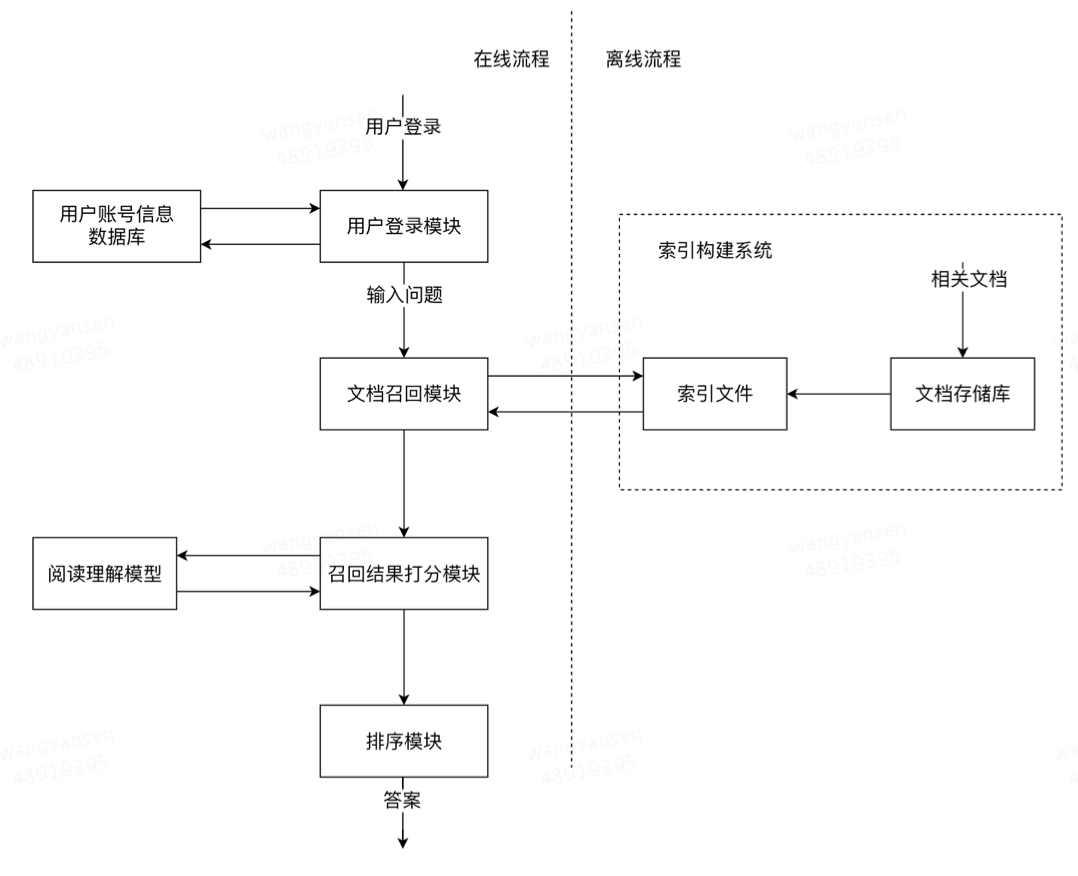
\includegraphics[scale=0.4]{fig/QA.png}
		\caption{问答需求\label{fig:QA}}
	\end{minipage}
	\qquad
	\begin{minipage}[t]{0.5\textwidth}
		\centering
		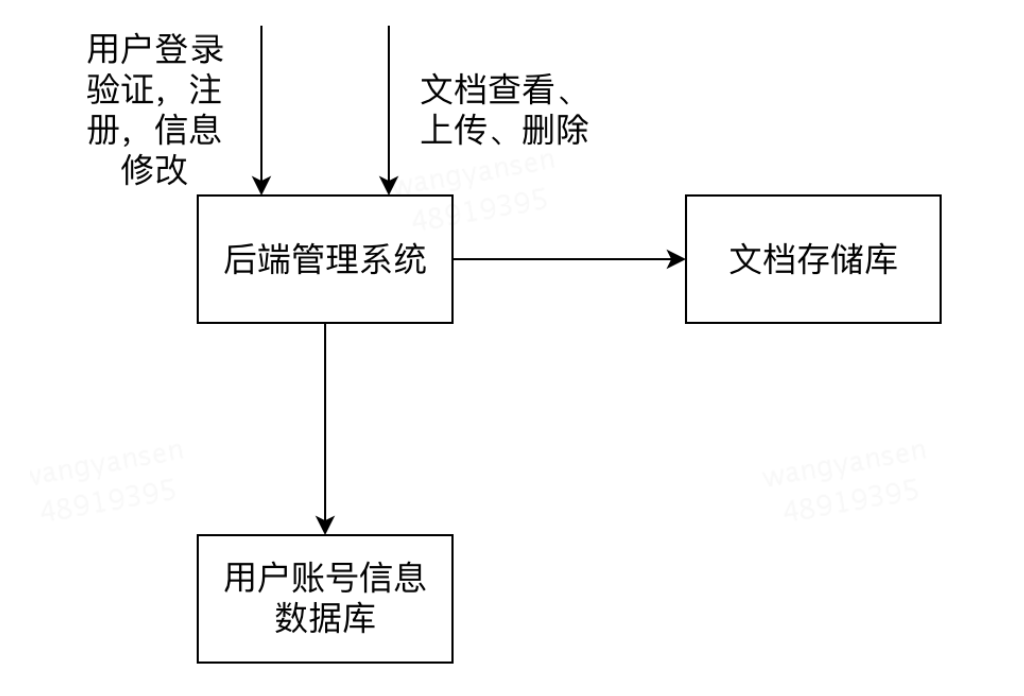
\includegraphics[scale=0.4]{fig/Manage.png}
		\caption{管理需求\label{fig:Manage}}
	\end{minipage}
\end{figure}


\subsection{问答需求}
\label{sec:req1}
在问答需求方面,前端需要完成搜索框的设计、搜索结果列表的展示,并与后端相应的接口进行对接。

后端则需要将文档数据库、索引系统和阅读理解模型串联起来,使得前端输入一个问题,后端可以从索引系统中快速检索出相应的文档,并将检索到的文档和问题发送给阅读理解模型,阅读理解模型从检索到的文档中抽取出问题对应的答案。

\subsection{文档与用户管理需求}
\label{sec:req2}
在文档和用户管理方面,前端需要完成管理页面的设计,并与后端接口通信。后端需要在数据库中存储所有的文档和用户信息,并且响应前端对文档增删改以及对用户信息修改的需求。

此外,当进行文档增删改的时候,索引系统需要监听到数据库文档的变动,并将索引系统中的文档与数据库的文档进行同步。

\section{项目架构}  % 任一
本项目的整体架构如图~\ref{fig:structure}所示。前端框架选用Vue.js,后端框架选用Django。索引系统选择Elastic Search,阅读理解模型是美团提供的。具体的项目功能,已经在~\ref{sec:req1}和~\ref{sec:req2}中叙述了,此处不再重复。

% one picture
\begin{figure}[htbp]  % htbp是插入图片的位置参数,直接用就好
    \centering  % 使图片居中
    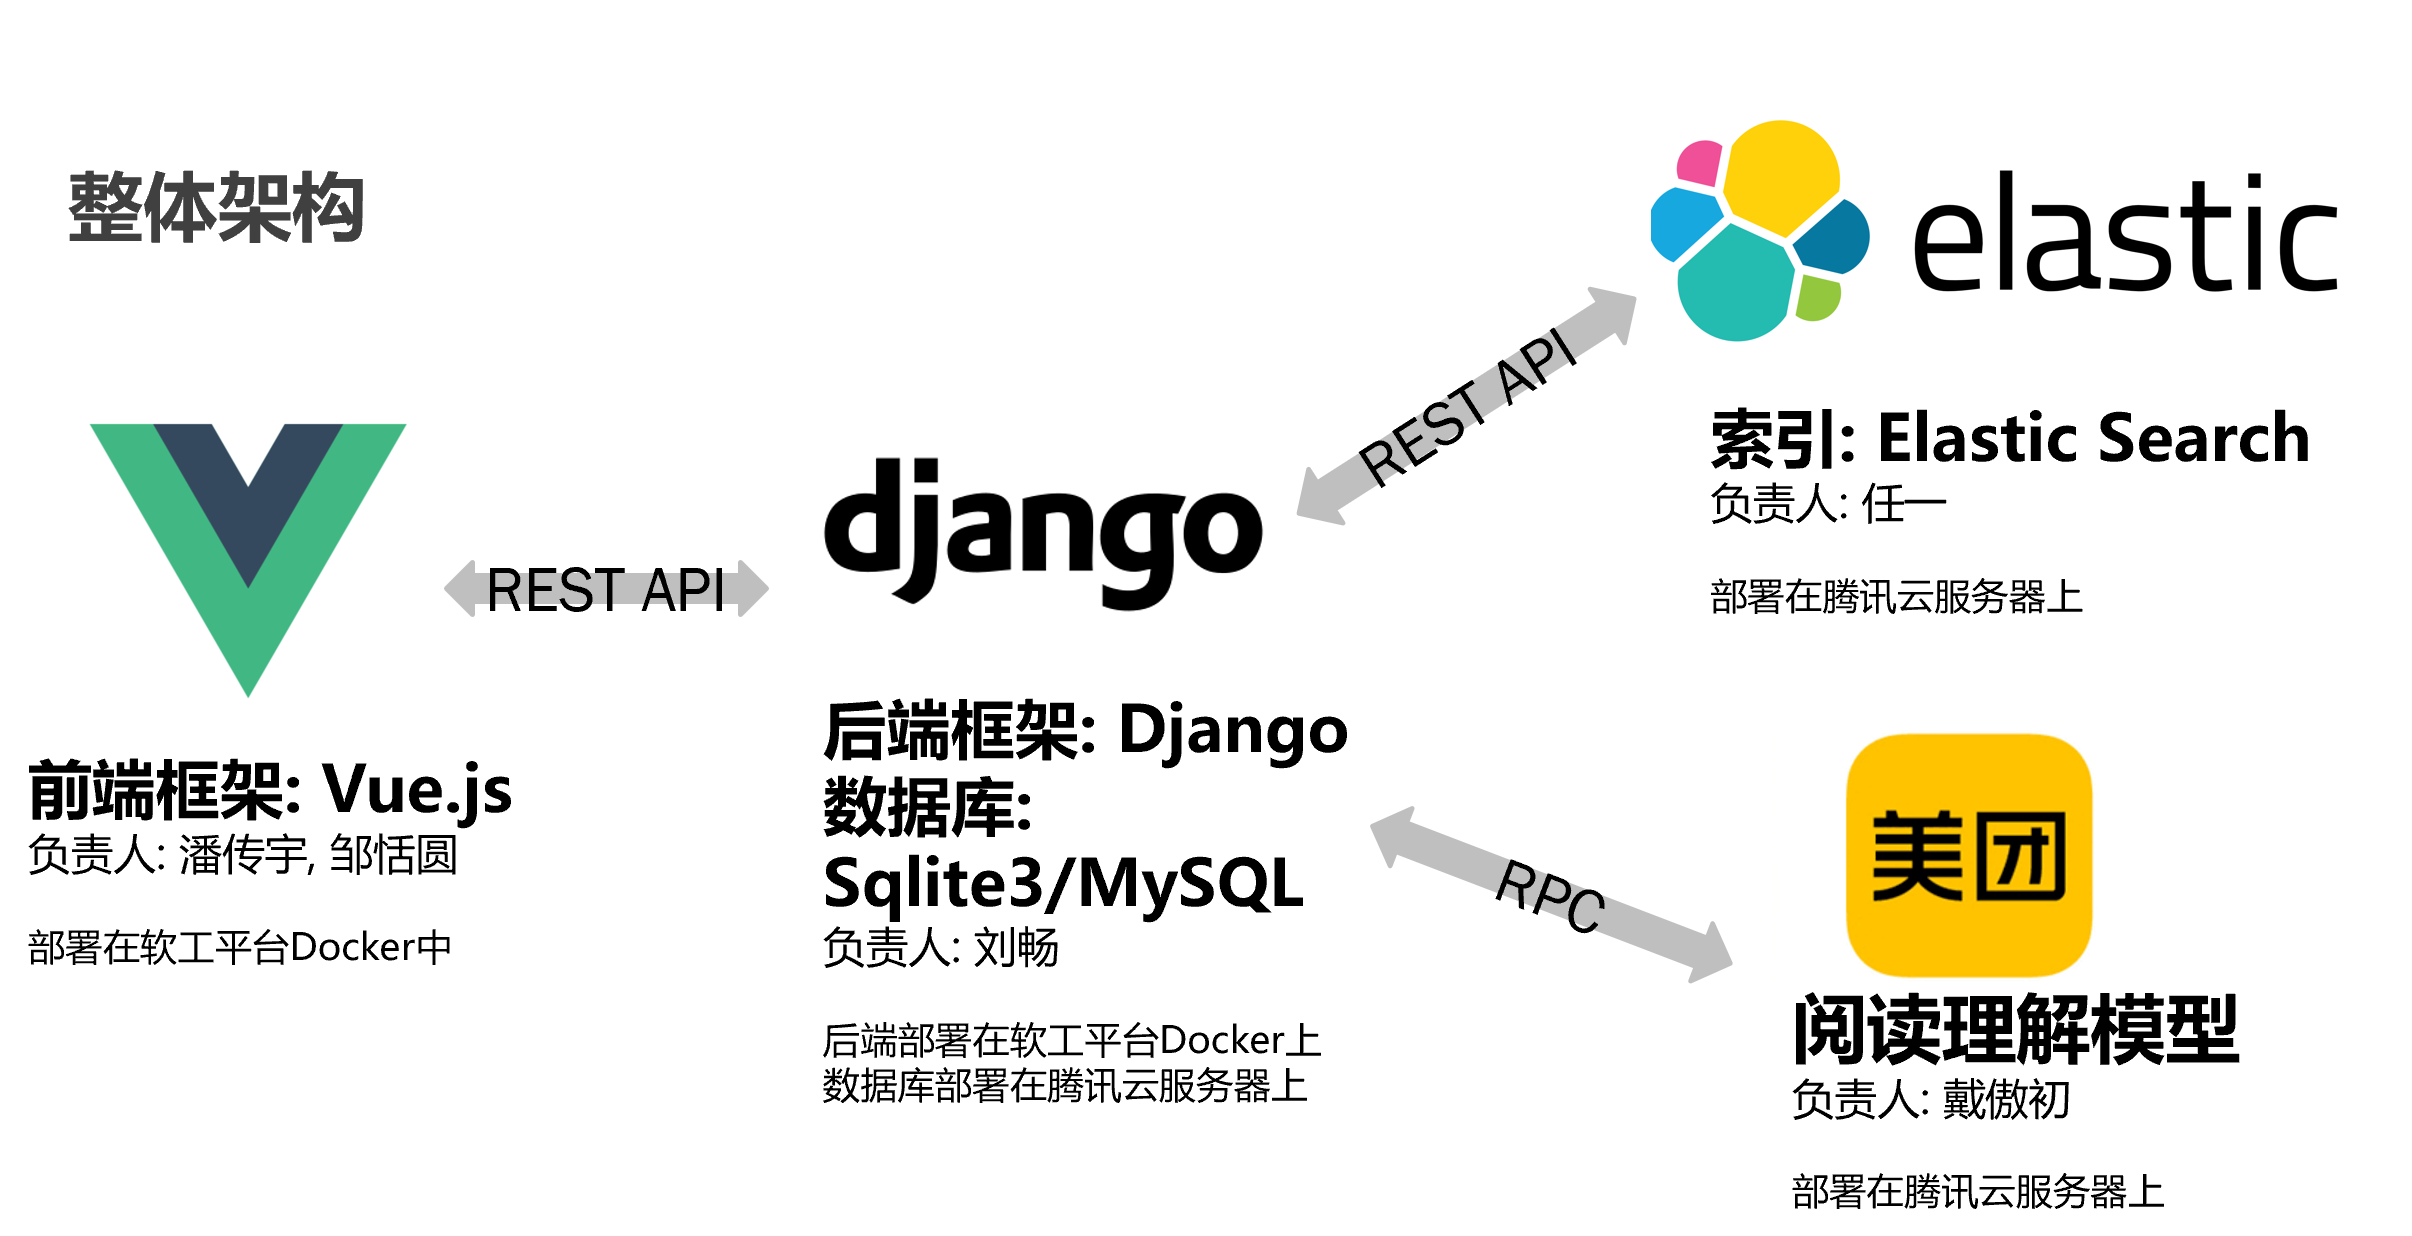
\includegraphics[width=0.8\textwidth]{fig/structure.png}  % 这里设定了图片的大小和路径
    \caption{项目整体架构}  %  图片的标题
    \label{fig:structure}  % 图片的label,方便在文中引用
\end{figure}
    

\section{模块和接口设计}
\subsection{前端}  % 潘传宇、邹恬圆
\subsubsection{整体架构}
前端使用Vue框架完成。不同的页面各自设为一个view;不同页面内的相同组件通过组件复用的方式完成复用。

前端与后端通信的接口严格意义上仅有两个,如下:
\begin{lstlisting}
fetch(url, param, show_text, cookie={withCredentials: true})
post(url, data={}, cookie={withCredentials: true})
\end{lstlisting}

两个接口内调用axios库中的get和post函数,将参数通过HTTP协议传递给后端,参数的放置严格依照HTTP协议的规定。

前端页面仅需要根据自身当前的状态和用户的交互动作判断用户的交互意图,然后给正确的后端发送HTTP请求并接受、展示后端发来的相应。

由于本项目中前端和后端是分离的,所以涉及到需要解决跨域请求的问题。项目中使用代理的方式完成跨域请求相关问题的解决。


\subsubsection{具体页面设计}

项目主要分为Home、QueryResult、User,About四个页面。User下包含UserInfo,History,Modify\_Doc和Upload\_Doc四个组成部分。此外还有Signin,Signup,SearchBar,TextItem等组件。

\myparagraph{Home和QueryResult页面}

QueryResult界面完成用户提出的问答需求的交互。搜索任务的发起逻辑由QueryResult vue提供。通过调用fetch接口向后端的/docs/search域名发送问题、请求回答完成主体逻辑。用户可以在搜索框中输入自己的问题并在发出搜索请求后收到后端返回的答案、答案来源全文和答案置信度评分。各条搜索结果均可展开或者收起,方便用户自行选择。Home界面同样拥有搜索框组件,方便用户简明快捷地开始问答流程。

\begin{figure}[htbp]  % htbp是插入图片的位置参数,直接用就好
    \centering  % 使图片居中
    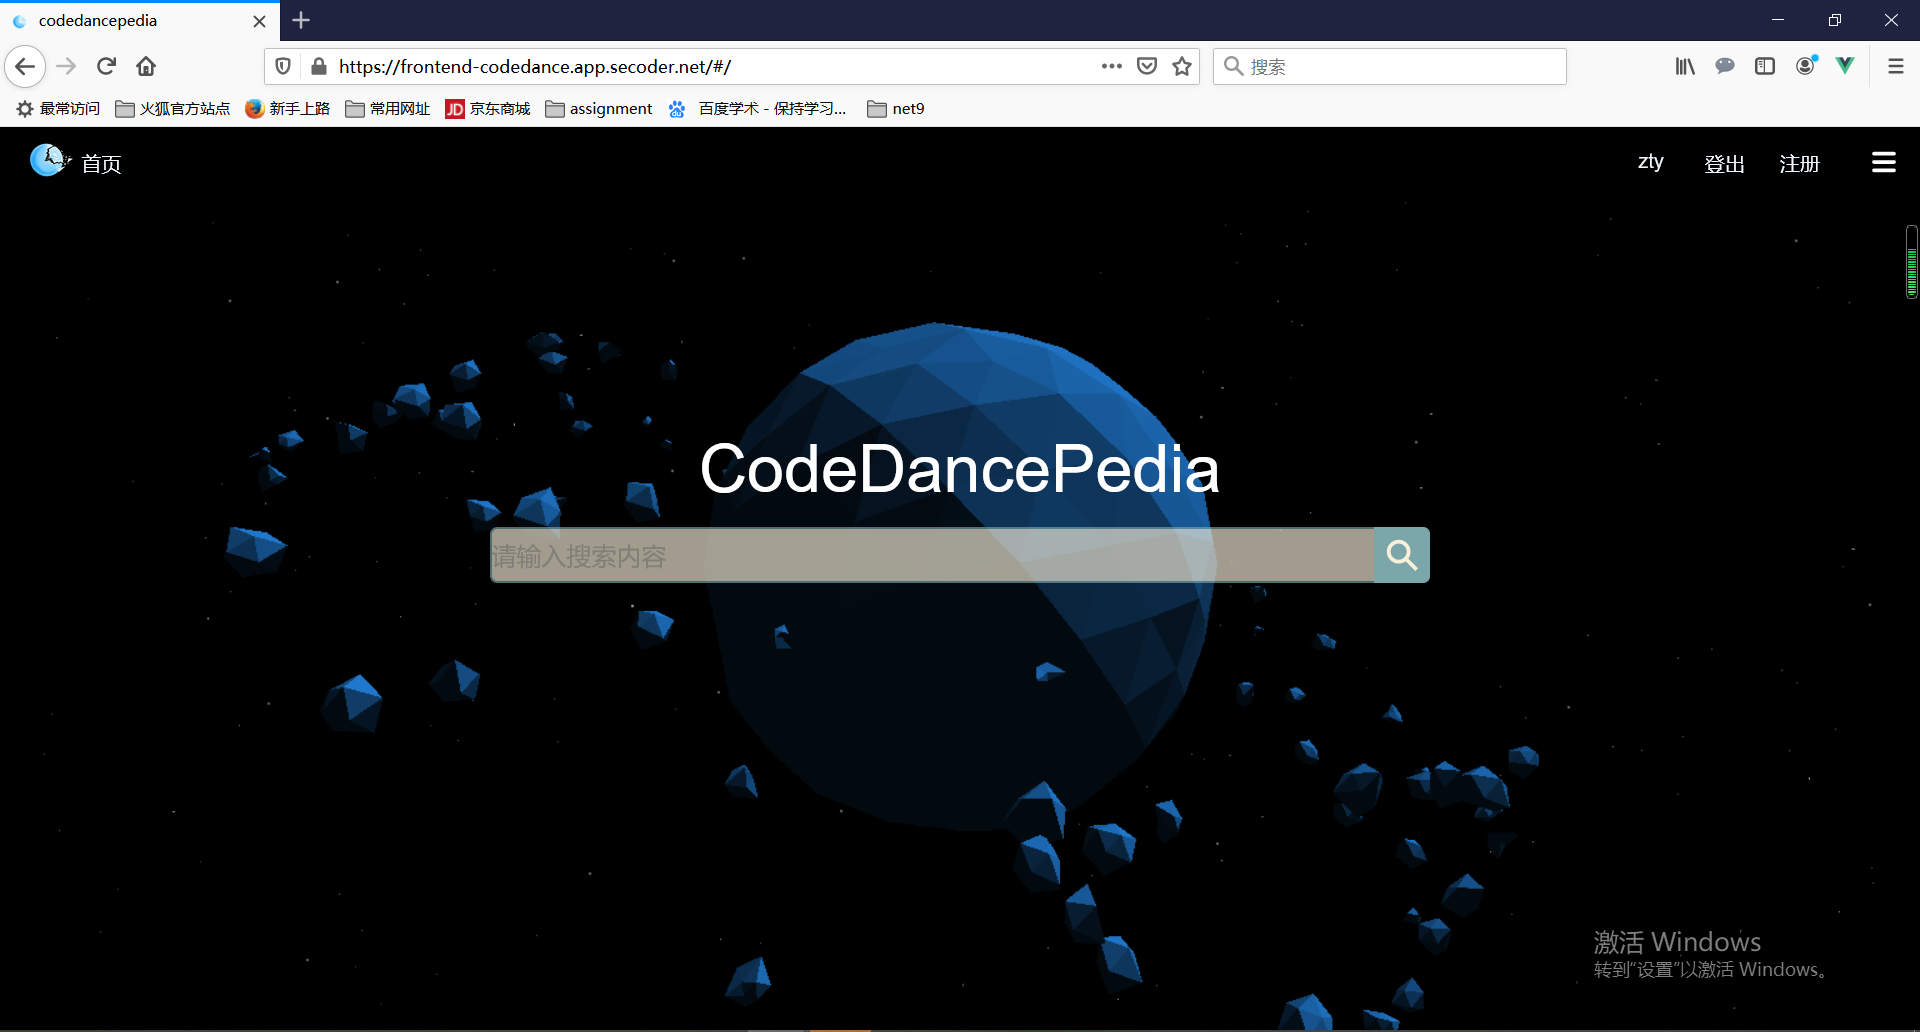
\includegraphics[width=0.8\textwidth]{fig/home.PNG}  % 这里设定了图片的大小和路径
    \caption{Home页面}  %  图片的标题
    \label{fig:structure}  % 图片的label,方便在文中引用
\end{figure}

\begin{figure}[htbp]  % htbp是插入图片的位置参数,直接用就好
    \centering  % 使图片居中
    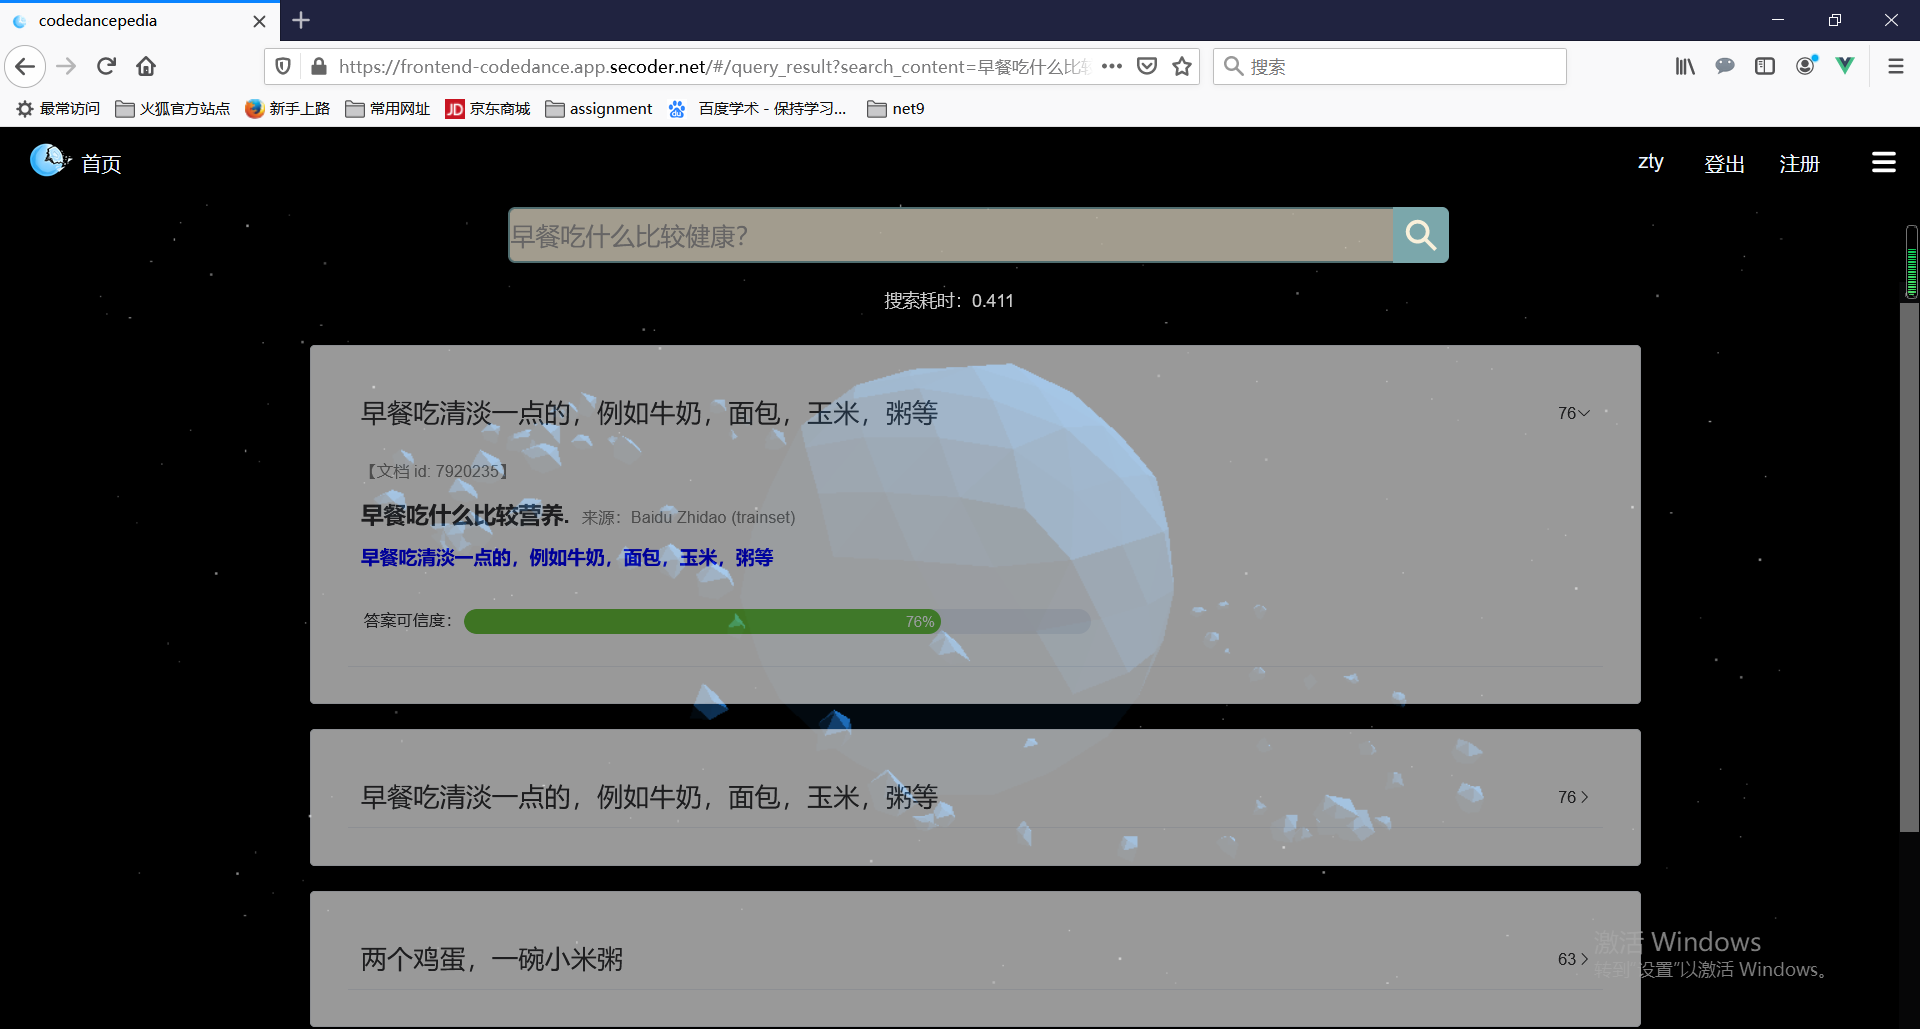
\includegraphics[width=0.8\textwidth]{fig/search1.PNG}  % 这里设定了图片的大小和路径
    \caption{QueryResult页面成功搜索到合适回答}  %  图片的标题
    \label{fig:structure}  % 图片的label,方便在文中引用
\end{figure}

\myparagraph{signin/signup页面}

signin和signup界面完成用户的登录和注册操作。在注册页面中,用户需填写用户名和密码,并再次确认密码,若信息合法即可成功注册;在登录界面中,用户只需输入正确的用户名和密码即可登录。这里我们做了前端和后端的双重校验,以确保用户信息的正确性。后端通信采用post函数向/user/login(登录)和/user/register(注册)域名发送post请求,通过user id和user name进行校验。

\begin{figure}[htbp]  % htbp是插入图片的位置参数,直接用就好
    \centering  % 使图片居中
    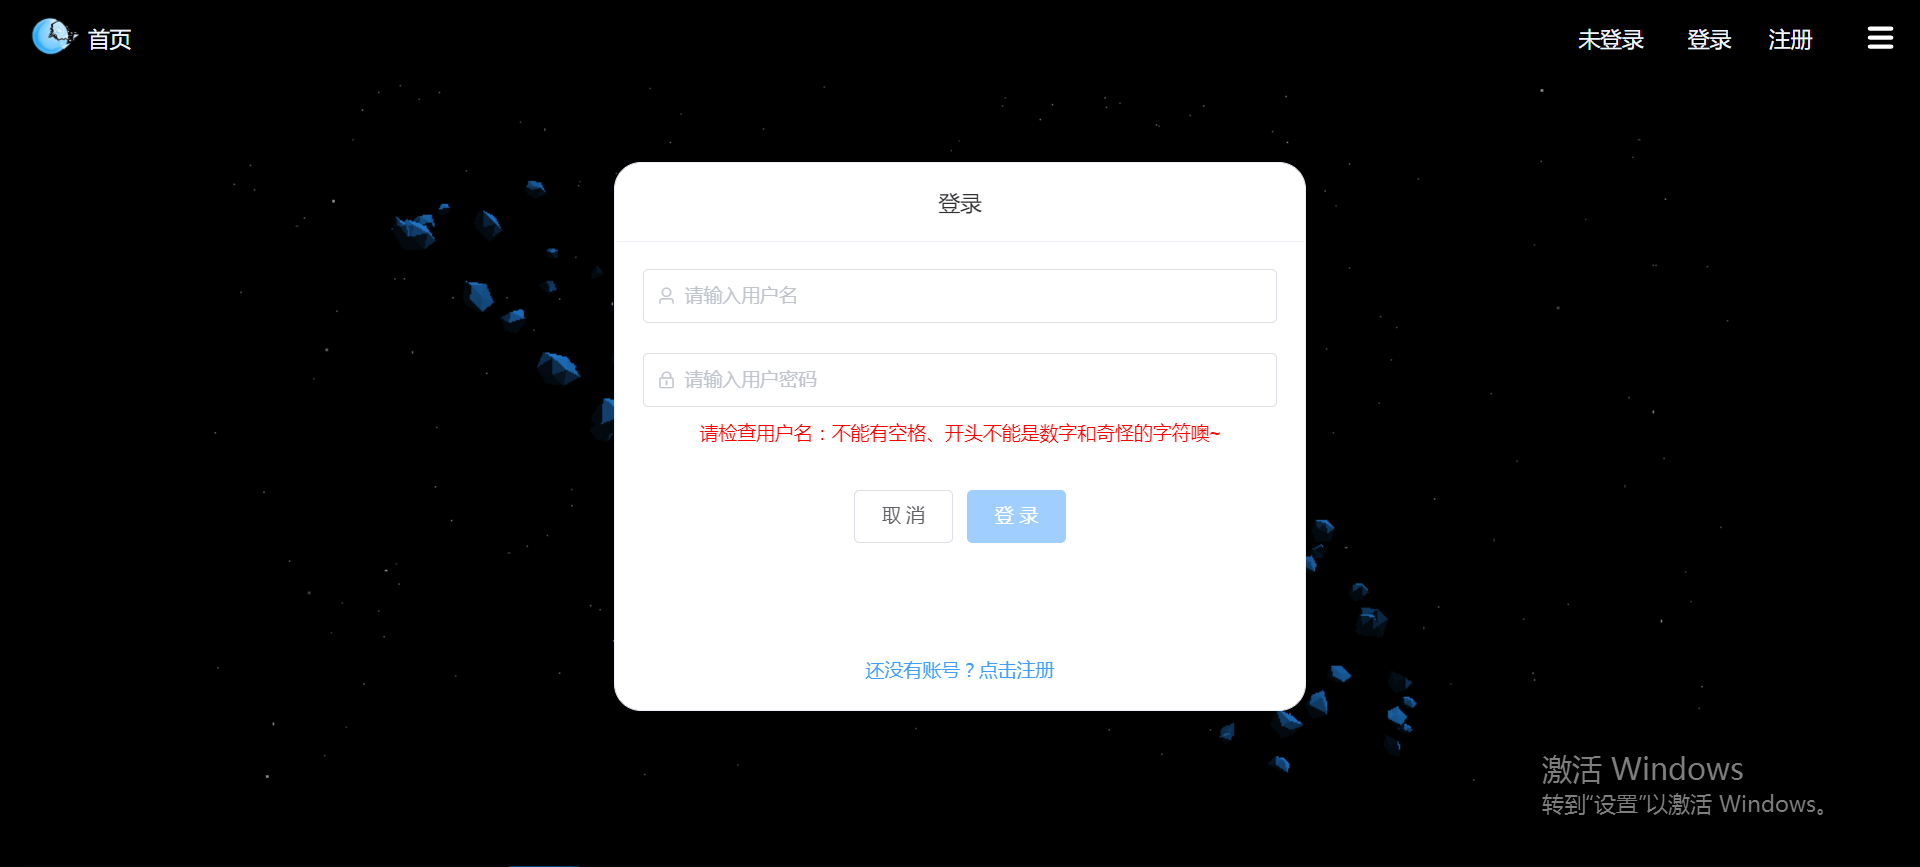
\includegraphics[width=0.8\textwidth]{fig/login.png}  % 这里设定了图片的大小和路径
    \caption{登录页面}  %  图片的标题
    \label{fig:structure}  % 图片的label,方便在文中引用
\end{figure}

\begin{figure}[htbp]  % htbp是插入图片的位置参数,直接用就好
    \centering  % 使图片居中
    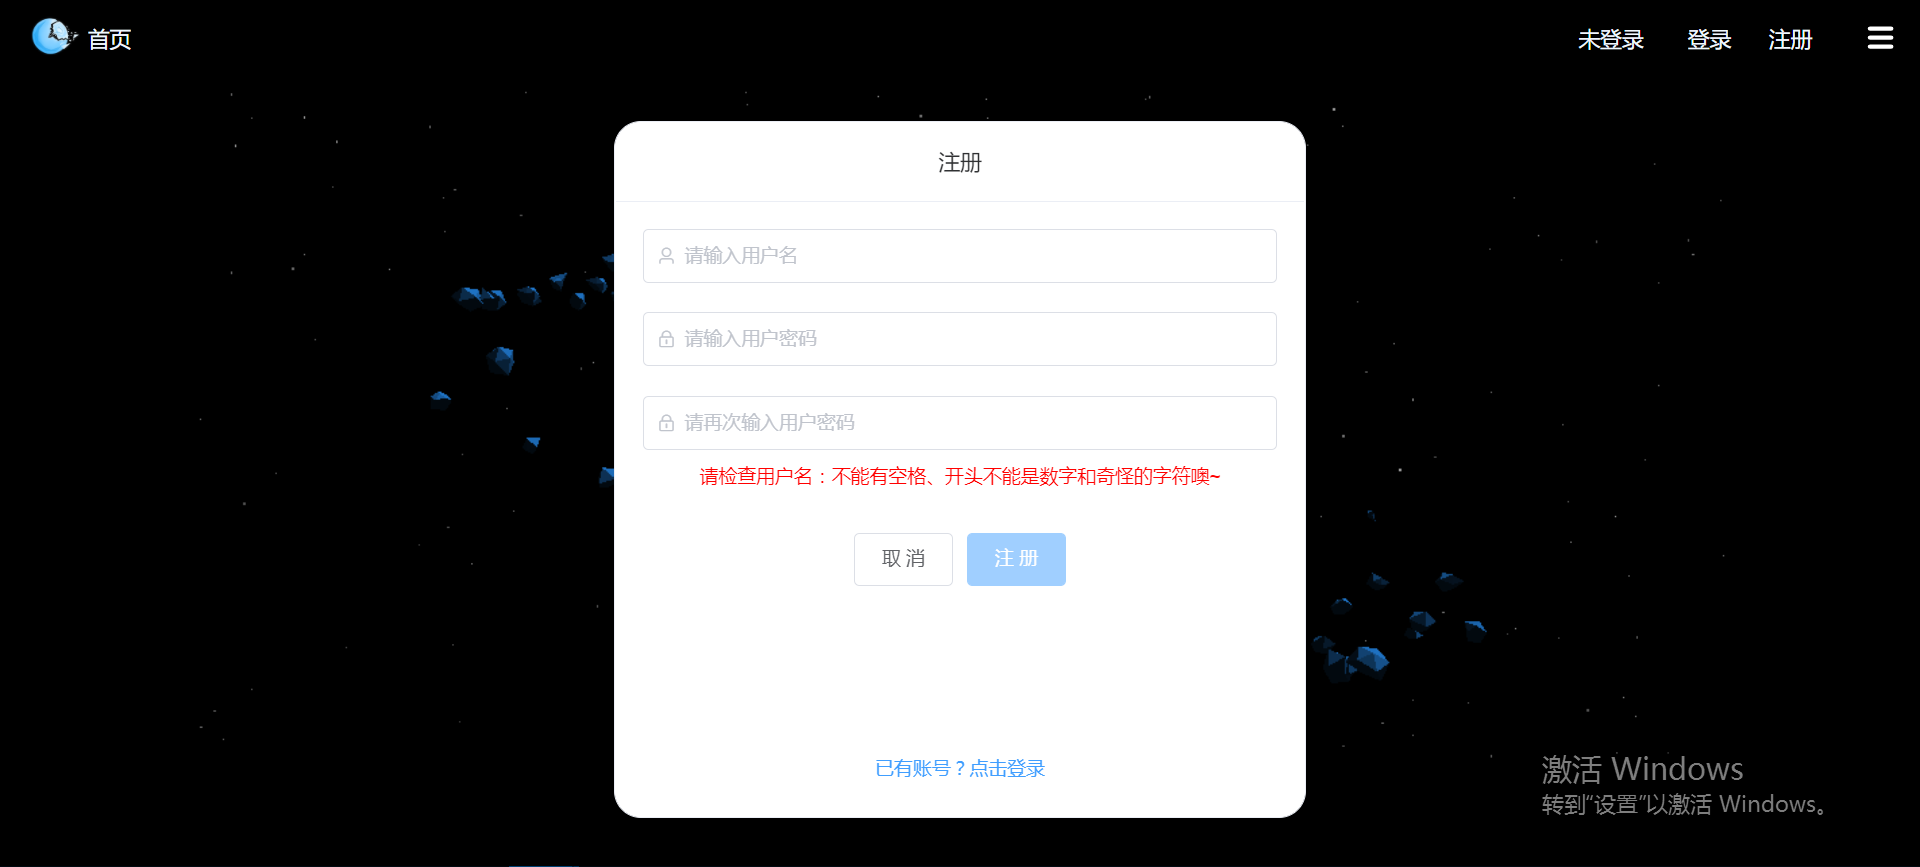
\includegraphics[width=0.8\textwidth]{fig/signup.png}  % 这里设定了图片的大小和路径
    \caption{注册界面}  %  图片的标题
    \label{fig:structure}  % 图片的label,方便在文中引用
\end{figure}

\myparagraph{User页面}

User界面提供用户和文档管理。用户登录后即可以自由浏览、修改自己的UserInfo界面,并在History界面浏览自己的提问历史记录。如果用户是管理员身份,则可以在Modify\_Doc界面修改、删除文档,在Upload\_Doc界面批量导入文档。

a) UserInfo界面在修改用户信息时通过调动post接口、上传自己信息来完成前端和后端的交互。其中,用户可修改自己的用户名、个性签名和密码,修改后在左侧的用户信息和导航栏中相应信息也会及时修改。

\begin{figure}[htbp]  % htbp是插入图片的位置参数,直接用就好
    \centering  % 使图片居中
    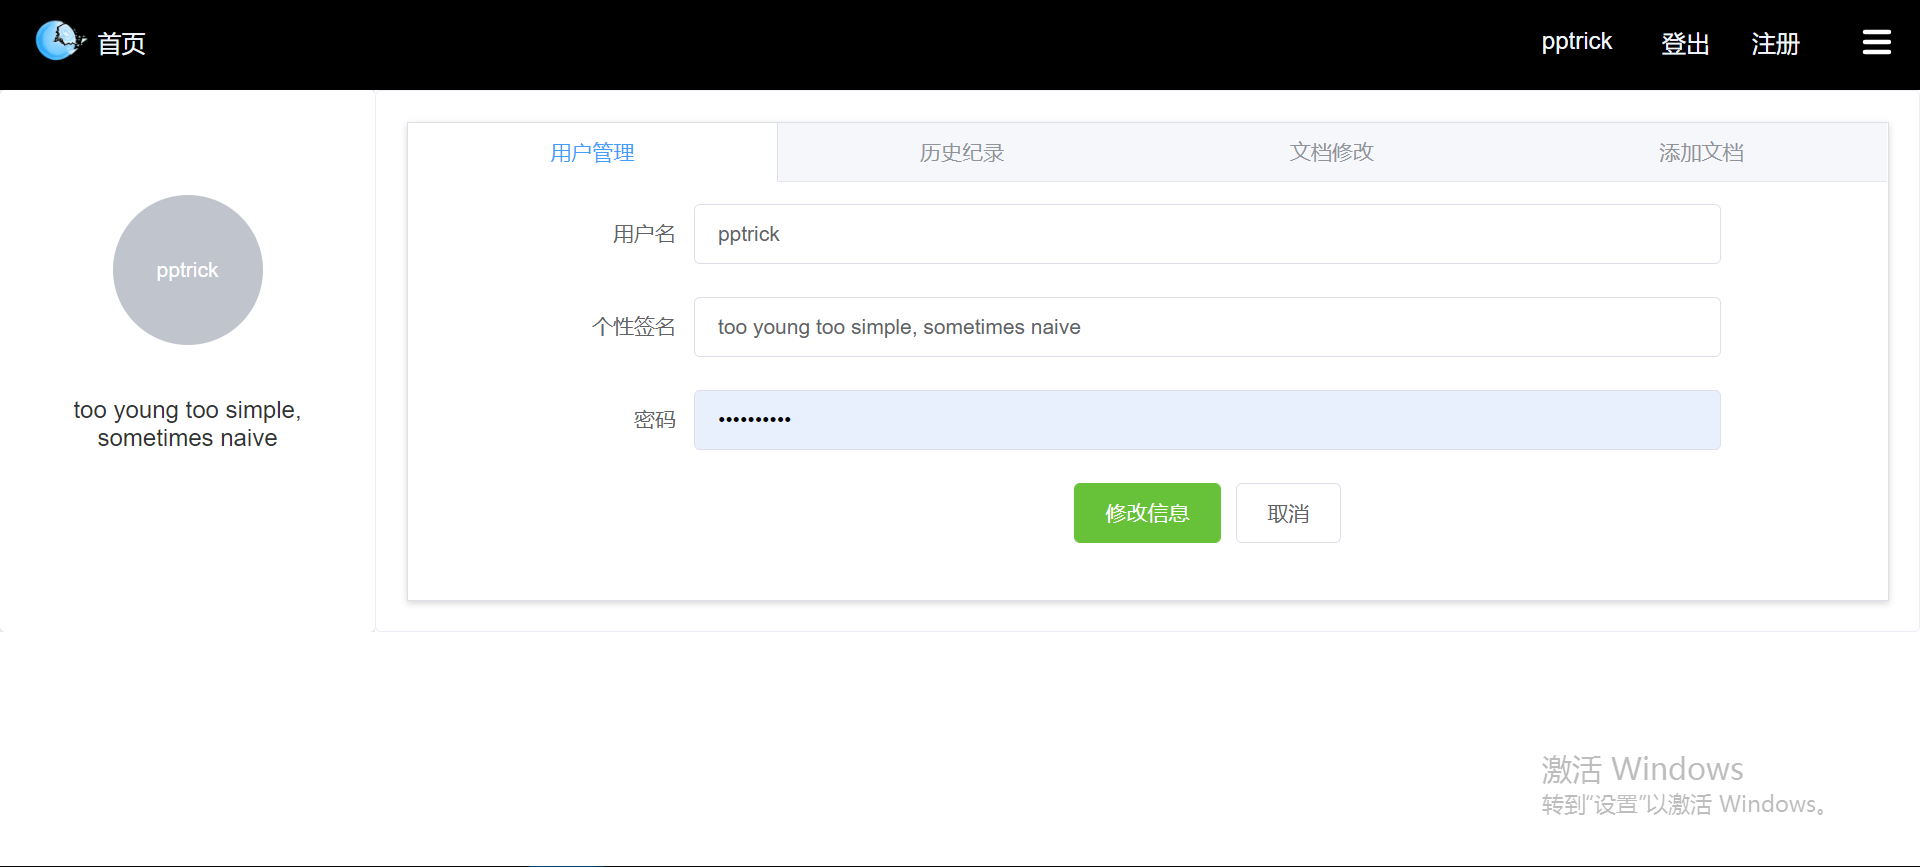
\includegraphics[width=0.8\textwidth]{fig/userinfo.png}  % 这里设定了图片的大小和路径
    \caption{UserInfo页面}  %  图片的标题
    \label{fig:userinfo}  % 图片的label,方便在文中引用
\end{figure}

b) History界面在渲染时通过调用fetch函数向后端的/user/history域名发送get请求携带参数“history”字样,获取后端数据库中目前存储的所有历史记录。当用户点击“清楚历史记录”时,通过弹窗确认用户不是误操作后,调用fetch函数向后端的/user/history域名发送get请求,参数为“clearHistory”字样。

\begin{figure}[htbp]  % htbp是插入图片的位置参数,直接用就好
    \centering  % 使图片居中
    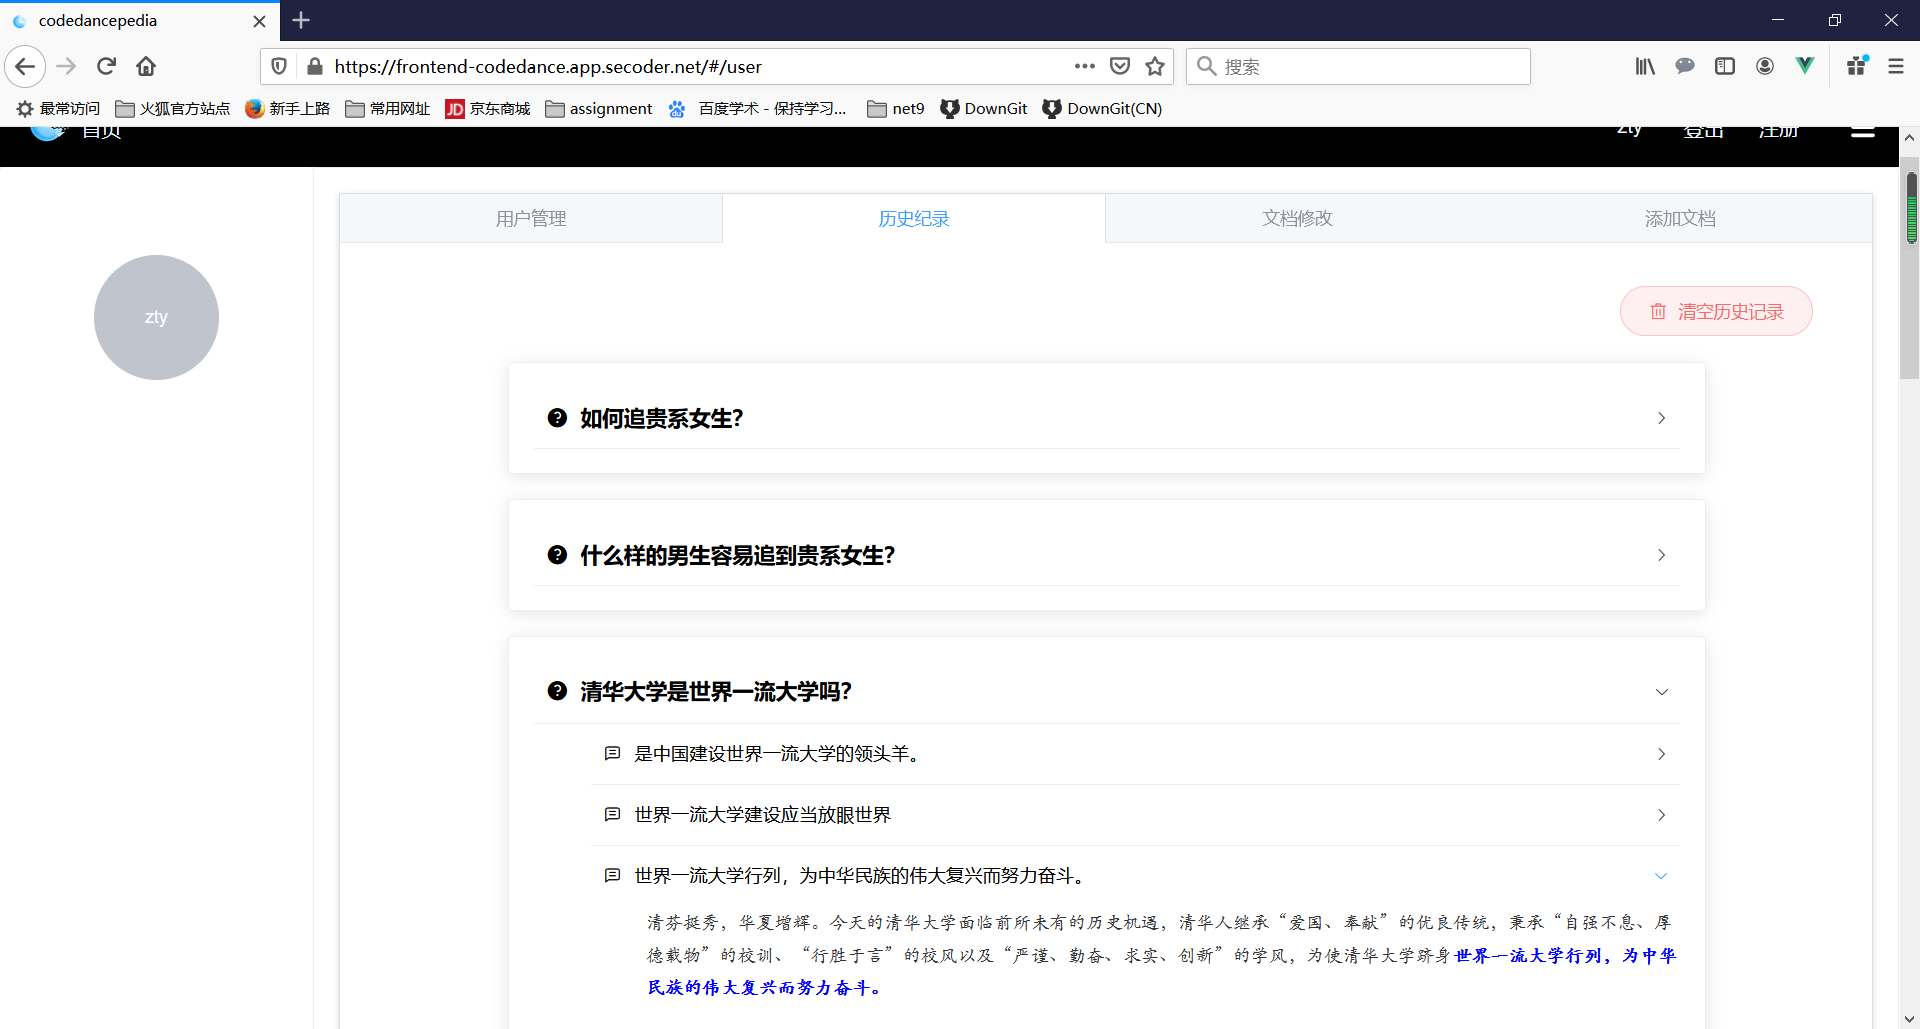
\includegraphics[width=0.8\textwidth]{fig/history2.PNG}  % 这里设定了图片的大小和路径
    \caption{History页面}  %  图片的标题
    \label{fig:structure}  % 图片的label,方便在文中引用
\end{figure}

c) Modify\_Doc页面支持文档按编号查找、修改、删除以及删除后恢复等操作。用户首先在编号框输入文档编号,回车后即可查找到对应文档;此时,用户可以针对召回的文档进行修改和删除操作。对于一篇已经删除的文档,在查找该篇文档时会有“已删除”提示,用户可以选择“恢复文档”将其恢复。该部分信息均通过post函数向后端的/docs/modify域名发送post请求,并在type字段中标识操作类型。

\begin{figure}[htbp]  % htbp是插入图片的位置参数,直接用就好
    \centering  % 使图片居中
    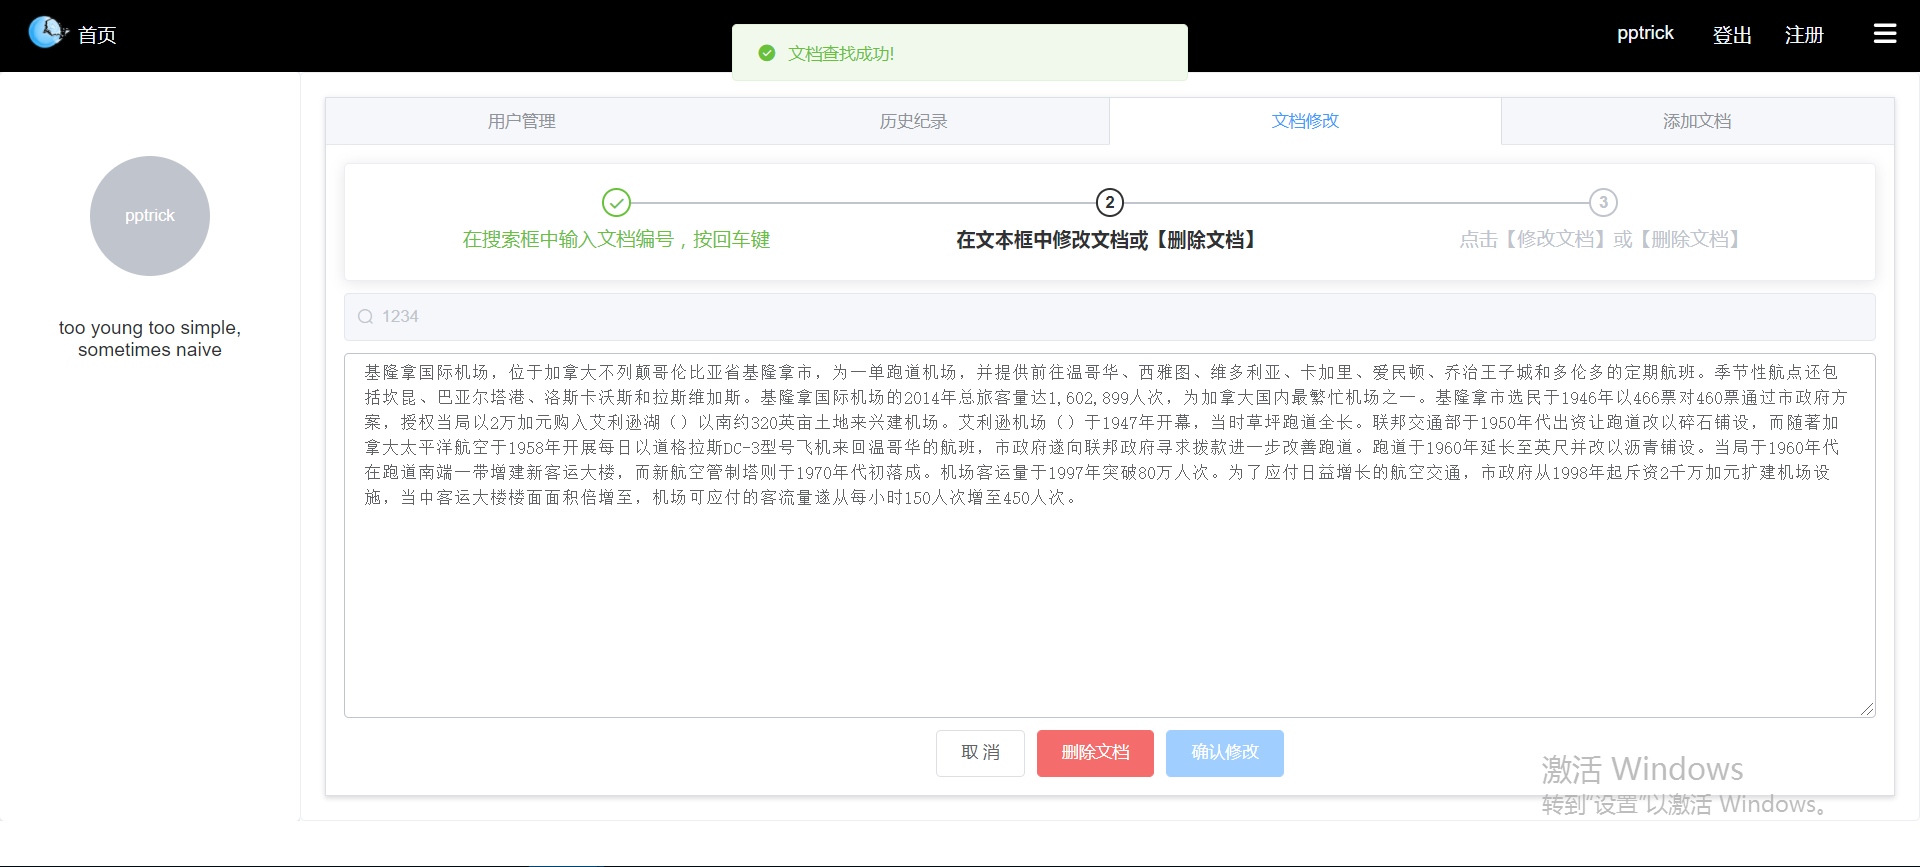
\includegraphics[width=0.8\textwidth]{fig/modify_doc.png}  % 这里设定了图片的大小和路径
    \caption{Modify\_Doc页面}  %  图片的标题
    \label{fig:modify_doc}  % 图片的label,方便在文中引用
\end{figure}

d) Upload\_Doc页面支持文件的批量上传。用户可以先在界面的模板下载连接上下载上传文档的模板即可通过上传一个文件来上传所有所有需要加入的文档。也支持同时上传多篇文档。上传功能使用ElementUI库中的El-upload组件原生上传接口完成。每个上传的文件都会返回相应的成功与否的信息和失败原因。上传成功的文件名会显示在页面左侧,同时看到文件中所含文档对应的文档id编号范围,方便后续查阅。已上传文档的记录保存在前端,因为后端不需要知道这篇文档是由哪个管理员加入的,不需要持久化存储,因此退出页面后相应信息丢失。
\begin{figure}[H]
	\begin{minipage}[t]{0.5\textwidth}
		\centering
		\includegraphics[scale=0.2]{fig/upload_download.PNG}
		\caption{模板下载\label{fig:onlycontent}}
	\end{minipage}
	\qquad
	\begin{minipage}[t]{0.5\textwidth}
		\centering
		\includegraphics[scale=0.2]{fig/upload_fail-2-1.PNG}
		\caption{文档上传结果示例\label{fig:titleandcontent}}
	\end{minipage}

\end{figure}

\myparagraph{About界面}

About界面是我们项目的介绍页面,里面有关于我们的项目以及团队的介绍,同时通过“走马灯”形式展示我们在开发过程中的一些精彩瞬间。

\begin{figure}[htbp]  % htbp是插入图片的位置参数,直接用就好
    \centering  % 使图片居中
    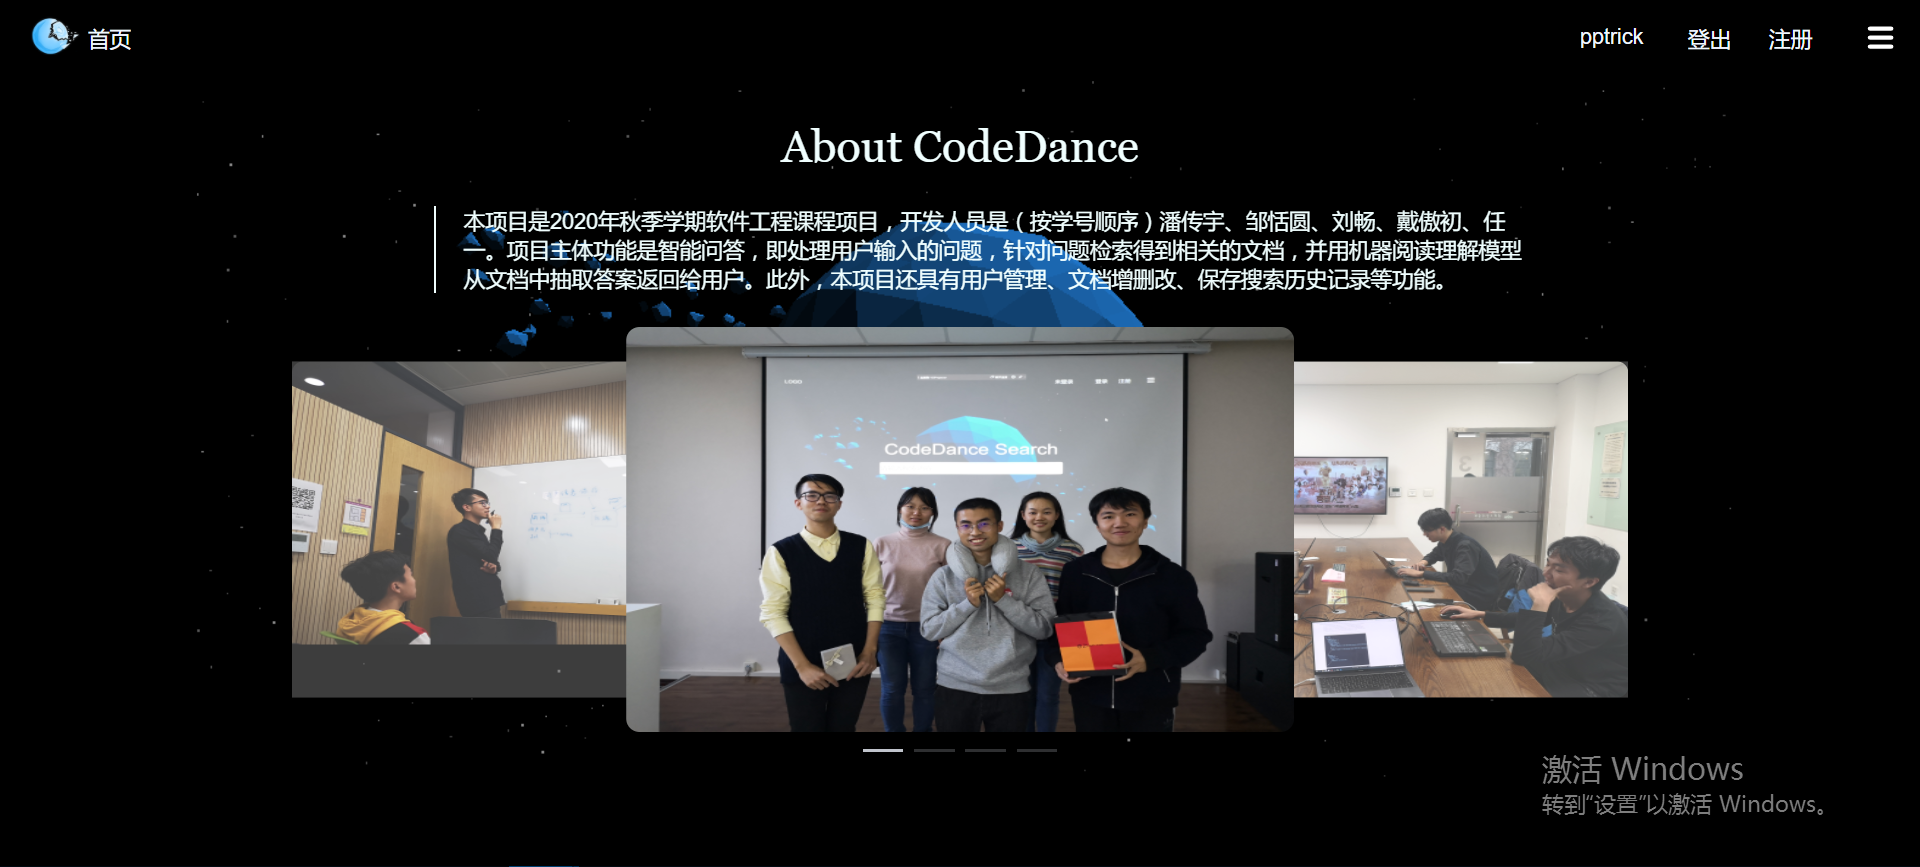
\includegraphics[width=0.8\textwidth]{fig/about.png}  % 这里设定了图片的大小和路径
    \caption{About页面}  %  图片的标题
    \label{fig:about}  % 图片的label,方便在文中引用
\end{figure}

\subsection{数据库}  % 刘畅
\subsubsection{结构设计}
数据库数据主要分为两个部分:用户信息和文档信息。
\myparagraph{用户信息}
\indent 本项目中不同需求对应用户信息表manage\_user\_user的不同字段,具体如表~\ref{tab:manage-user-user}:
% Please add the following required packages to your document preamble:
% \usepackage{multirow}
\begin{table}[h]
\caption{用户信息表设计}
\label{tab:manage-user-user}  % 表格的label,方便在文中引用
\centering
\begin{tabular}{|c|c|}
\hline
需求                       & 相关字段        \\ \hline
\multirow{3}{*}{注册/登录验证} & id          \\ \cline{2-2} 
                         & username    \\ \cline{2-2} 
                         & password    \\ \hline
\multirow{2}{*}{个人信息}    & bio         \\ \cline{2-2} 
                         & email       \\ \hline
历史记录                     & query\_json \\ \hline
\multirow{6}{*}{用户管理}    & is\_delete  \\ \cline{2-2} 
                         & is\_active  \\ \cline{2-2} 
                         & is\_admin   \\ \cline{2-2} 
                         & create\_at  \\ \cline{2-2} 
                         & updated\_at \\ \cline{2-2} 
                         & last\_login \\ \hline
\end{tabular}
\end{table}
\newline
其中具体字段的实现,将在数据库设计部分详细阐述。

\myparagraph{文档信息}
\indent 本项目中不同需求对应的文档信息表manage\_doc\_document的不同字段,具体如表~\ref{tab:manage-doc-document}:
% Please add the following required packages to your document preamble:
% \usepackage{multirow}
\begin{table}[h]
\centering
\caption{文档信息表设计}
\label{tab:manage-doc-document}  % 表格的label,方便在文中引用
\begin{tabular}{|c|c|}
\hline
需求                                   & 相关字段    \\ \hline
\multirow{4}{*}{获取文档/修改文档/删除文档/上传文档} & id      \\ \cline{2-2} 
                                     & content \\ \cline{2-2} 
                                     & title   \\ \cline{2-2} 
                                     & src     \\ \hline
文档状态                                 & status  \\ \hline
\end{tabular}
\end{table}

其中具体字段的实现,将在数据库设计部分详细阐述。

\subsubsection{接口设计}
由于后端使用的是Django框架,因此将功能按照按照两大块进行分类,分别是用户管理和文档管理,并注册了两个应用,名为
manage\_user和manage\_doc,应用内部都是使用ORM方式进行组织的。

本项目的接口文档地址在\href{https://easydoc.xyz/doc/71410797/1dBoJWEJ/skvUSixD}{这里}。
其中包括了调用API的方法,请求参数、返回值等。

下面针对重点的几个接口实现进行详细说明。

\begin{itemize}
    \item {
register/login: 采用HTTP的Basic认证,仅仅通过明文传输的用户名和密码实现了用户身份验证。
后端API首先检查前端传来的字段是否完整,其次检查各字段数据本身是否合法,最后将新用户数据
存入数据库/从数据库中获取相应的用户信息,并给前端返回user\_id,完成登录功能。
    }
    \item {
modify: 支持管理员删除/修改/恢复文档三种操作。在一次操作中,首先输入待操作的document\_id,
前端会首先fetch该文档(并查询状态),如果是存在的状态,则在前端页面显示对应的文档内容,
并支持后续的修改和删除;如果是被删除的状态,则后端不允许再次进行删除和修改,但可以继续进行恢复操作。
    }
    \item {
upload: 支持管理员通过固定json格式上传文档。后端主要解析前端传输过来的字节流,然后解析出文档内容和文档标题存入数据库。
    }
    \item {
search: 前端传入问题,索引系统进行文档召回,并传给模型,模型处理后返回结果。后端得到结果后在另外的线程进行历史记录的存储。
    }
\end{itemize}

\subsection{索引}  % 任一
\subsubsection{工作原理}
ElasticSearch是一个分布式、RESTful 风格的搜索和数据分析引擎,可以提供快速的文档检索功能。

文档检索的主要原理是倒排索引,通过对文档进行分词,我们可以建立起某个词在哪些文档中包含的表,而非某个文档包含哪些词的表,这样就可以大大提高文档检索的效率。除了倒排索引,Elastic Search还支持文档与问题不同相关性系数的计算、支持对文档的多个字段进行匹配并调整权重(例如同时对文档 的标题和内容做匹配,并且认为标题的权重更大)等等丰富而强大的功能。


\begin{figure}[htbp]  % htbp是插入图片的位置参数,直接用就好
    \centering  % 使图片居中
    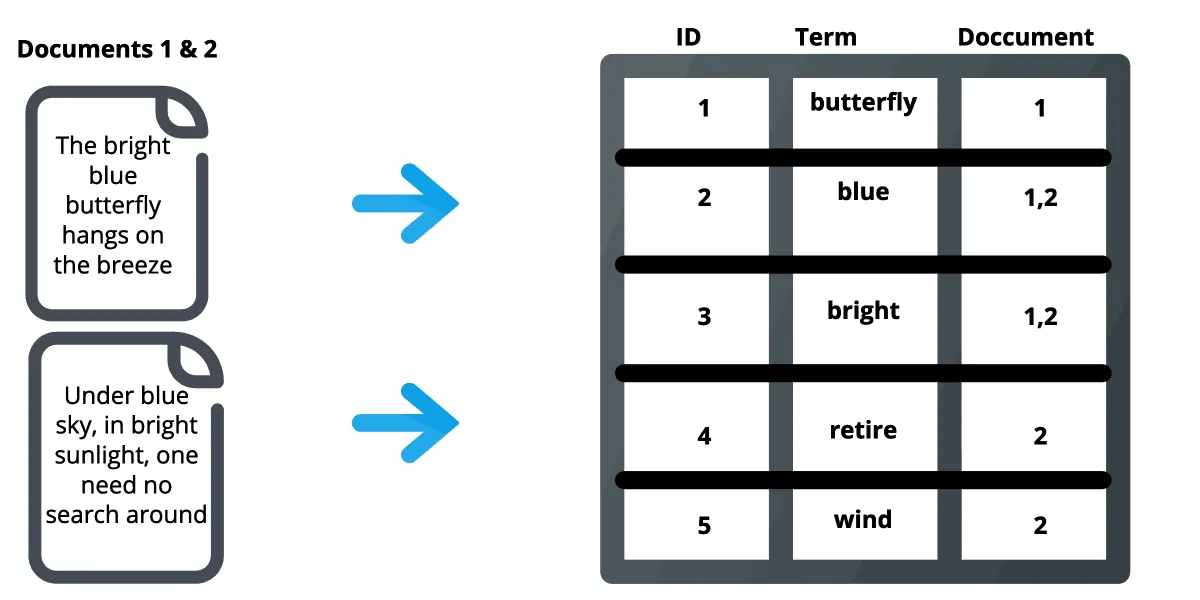
\includegraphics[width=0.7\textwidth]{fig/inverse-index.png}  % 这里设定了图片的大小和路径
    \caption{倒排索引基本原理}  %  图片的标题
    \label{fig:inverted-index}  % 图片的label,方便在文中引用
\end{figure}
    

\subsubsection{通信与接口设计}
索引系统在整个项目中,负责与后端数据库进行通信。在后端接受到前端的问题后,会调用ElasticSearch的检索函数,该函数可以返回检索到的文档,并给出每个文档与问题的相关系数等信息。

索引系统与后端数据库的通信(包括问题搜索、文档增删改同步),本项目中使用了Django Elasticsearch DSL这个开源库\footnote{Django Elasticsearch DSL的Github链接是\url{https://github.com/django-es/django-elasticsearch-dsl}}。
这个库有很方便的函数调用接口,以问题字符串作为输入,可以返回ElasticSearch检索到的文档及相关信息。

\subsubsection{效果评测}
索引系统的性能和各项指标,关乎整个项目的用户体验。下面我们从性能和Precision\&Recall的角度,展示索引系统评测的结果。

性能方面,Elastic Search在13000000篇文档上,同时匹配文档标题和内容时,返回的平均耗时上21.7ms,其中90\%的问答可以在38ms内返回,显示了索引系统强大的性能。

\begin{figure}[H]
	\begin{minipage}[t]{0.5\textwidth}
		\centering
		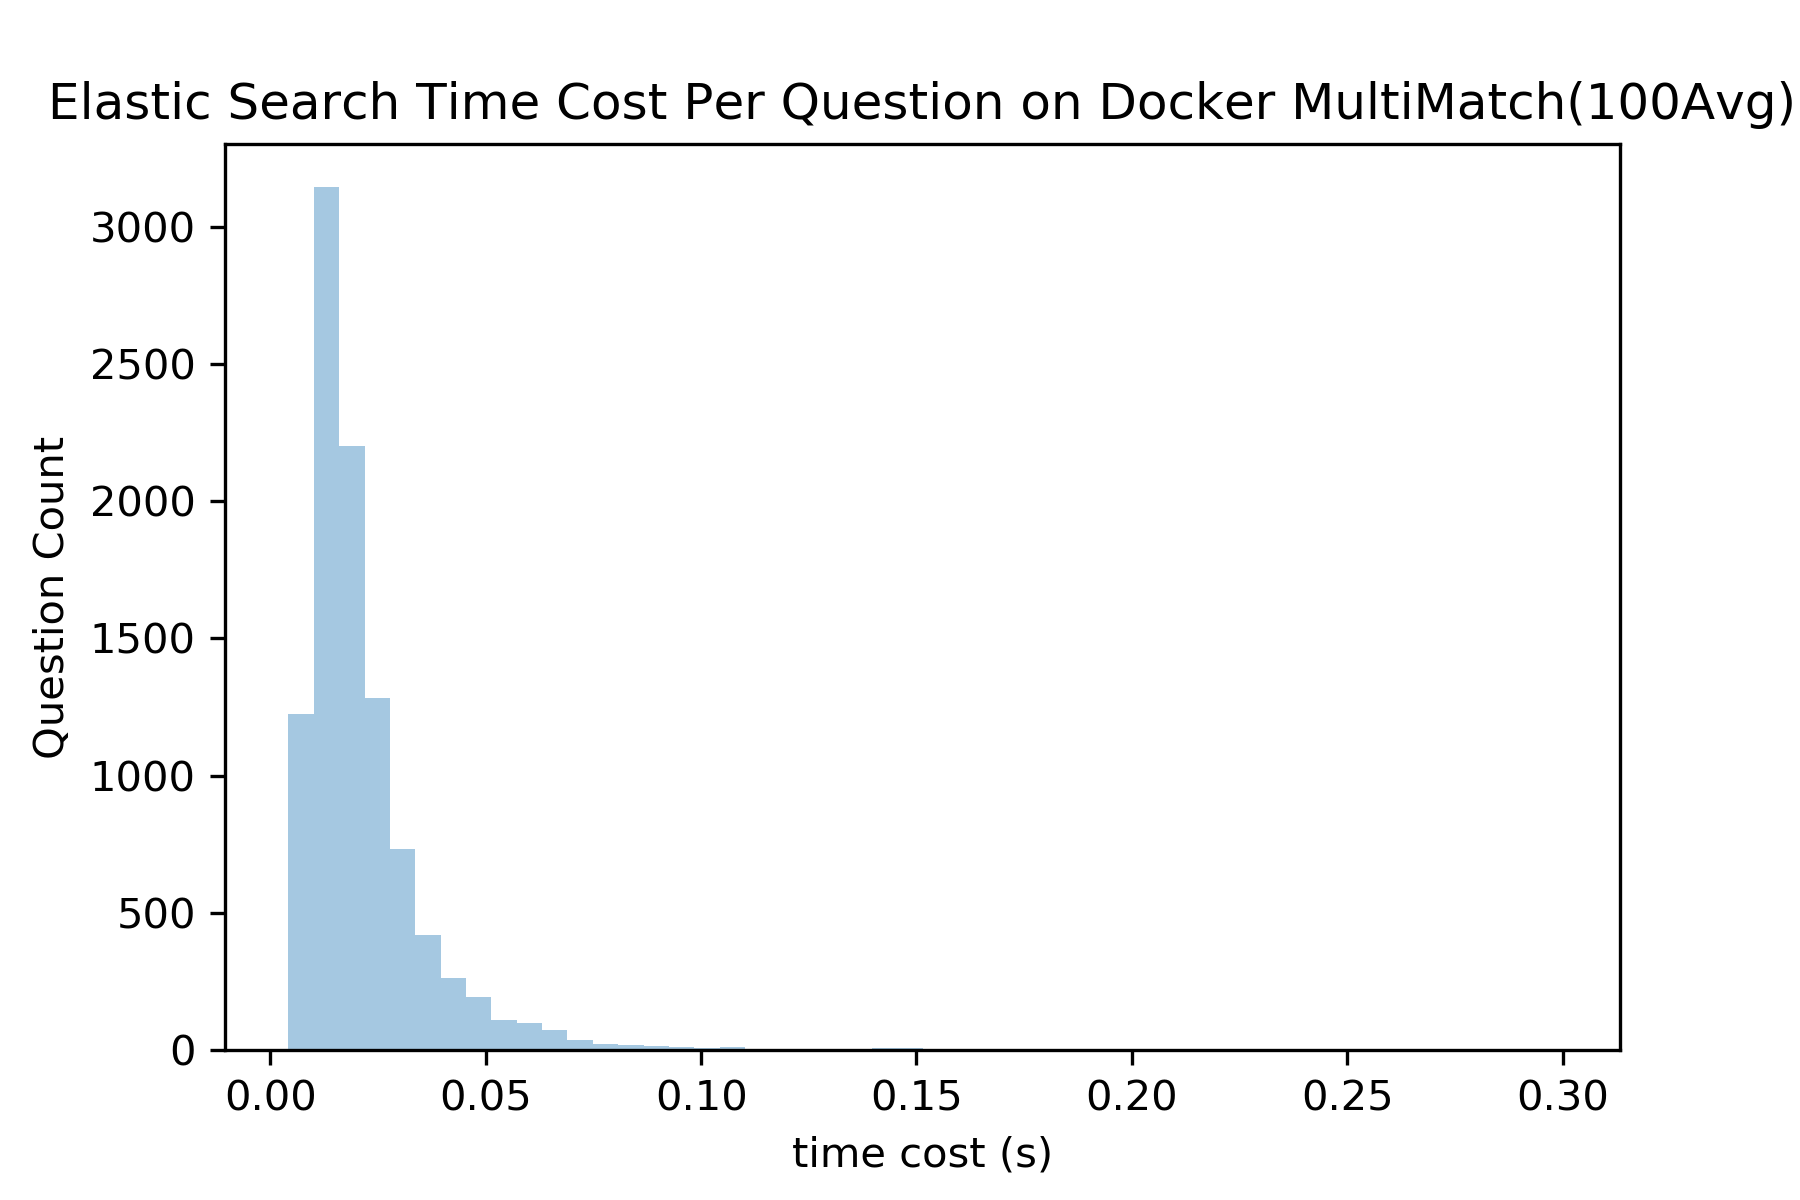
\includegraphics[scale=0.5]{fig/ESTIME.png}
		\caption{ElasticSearch检索耗时分布图\label{fig:estime}}
	\end{minipage}
	\qquad
	\begin{minipage}[t]{0.5\textwidth}
		\centering
		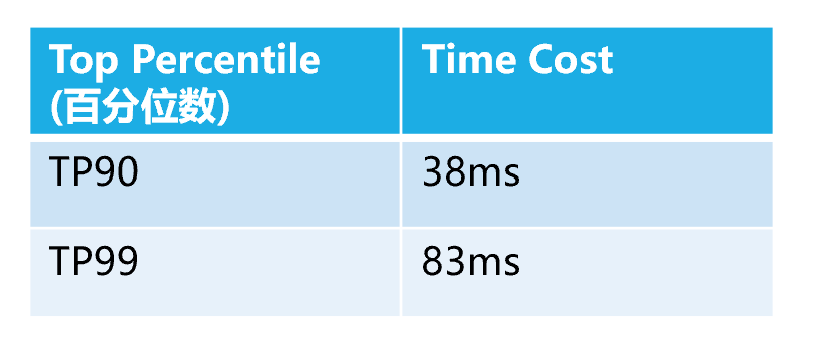
\includegraphics[scale=0.5]{fig/perc.png}
		\caption{ElasticSearch检索耗时百分位数\label{fig:percentile}}
	\end{minipage}
\end{figure}

在Precision\&Recall方面,我们对比了只匹配文档内容和对文档内容与标题都进行匹配的检索方法。
\begin{figure}[H]
	\begin{minipage}[t]{0.5\textwidth}
		\centering
		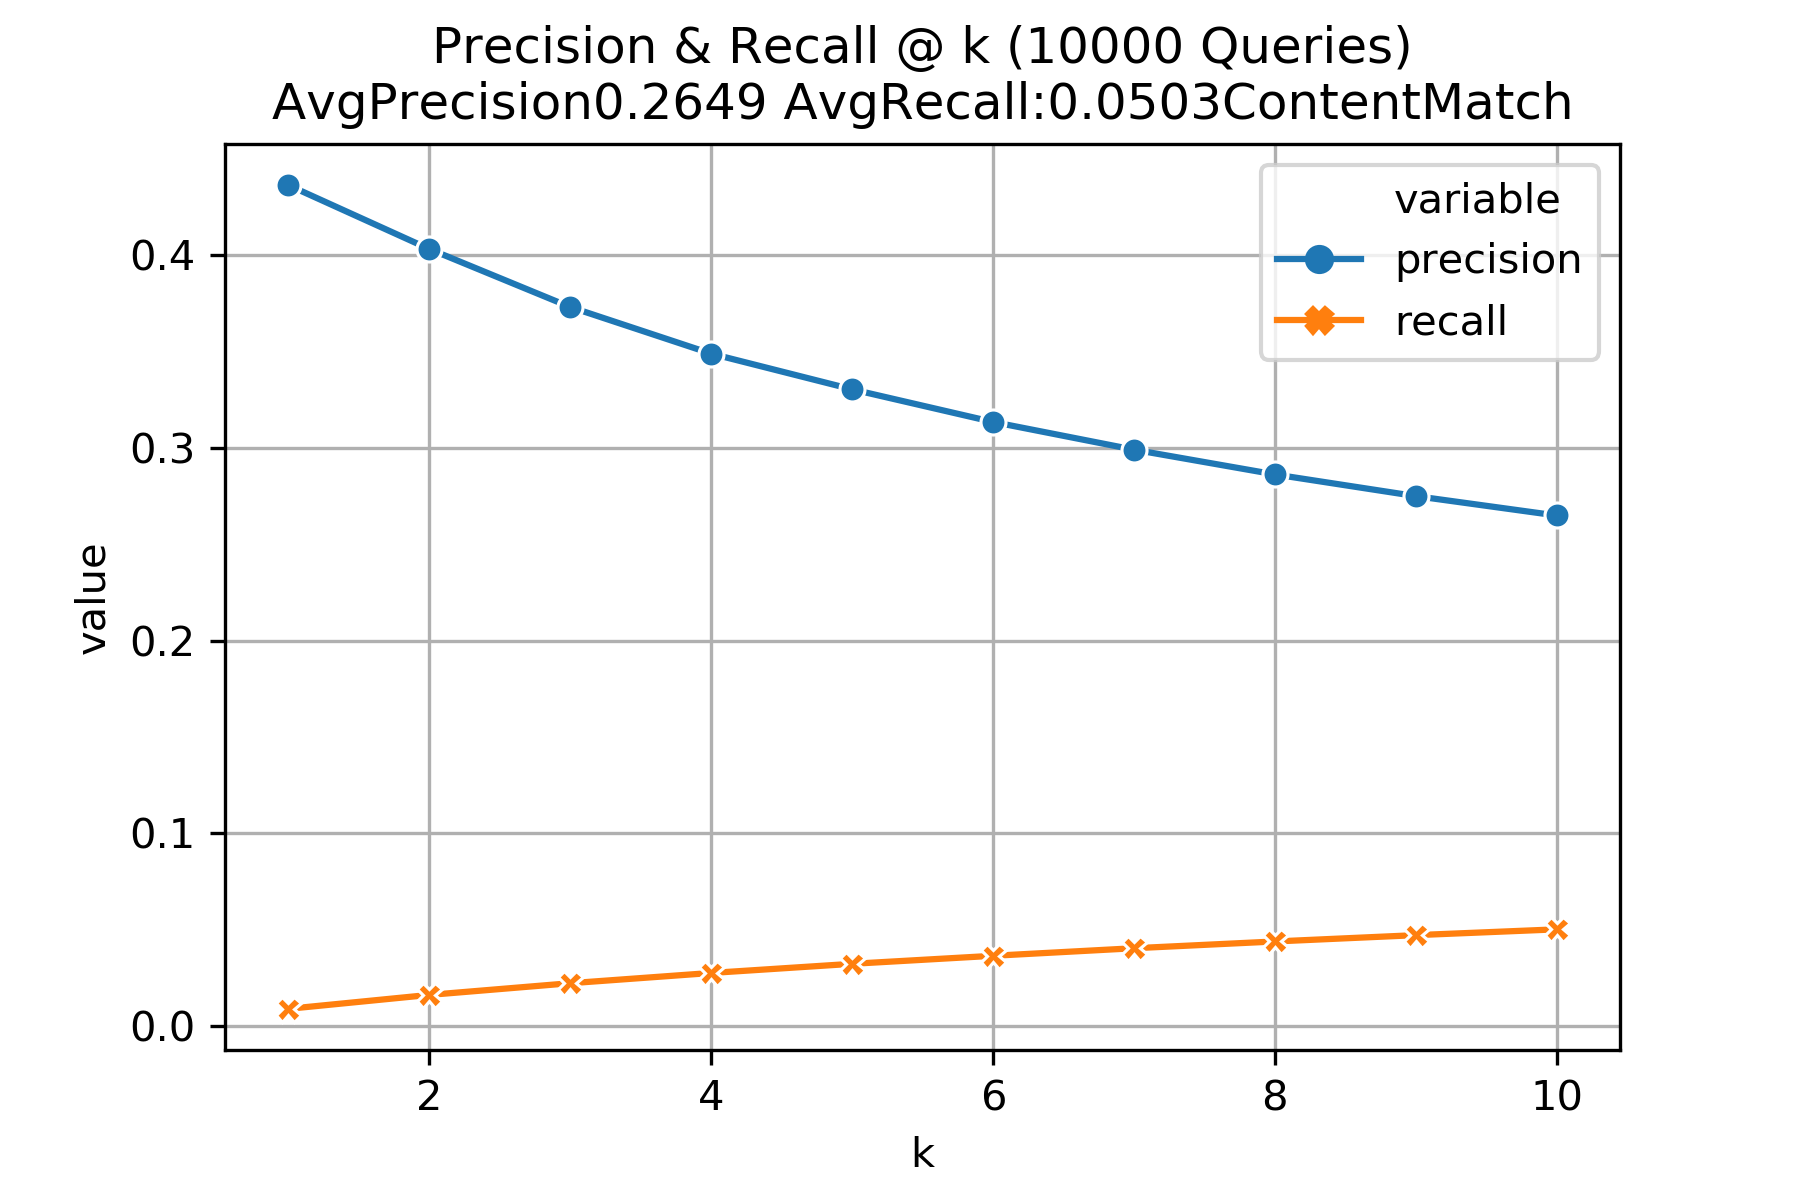
\includegraphics[scale=0.5]{fig/OnlyContent.png}
		\caption{只匹配文档内容的检索Precision和Recall\label{fig:onlycontent}}
	\end{minipage}
	\qquad
	\begin{minipage}[t]{0.5\textwidth}
		\centering
		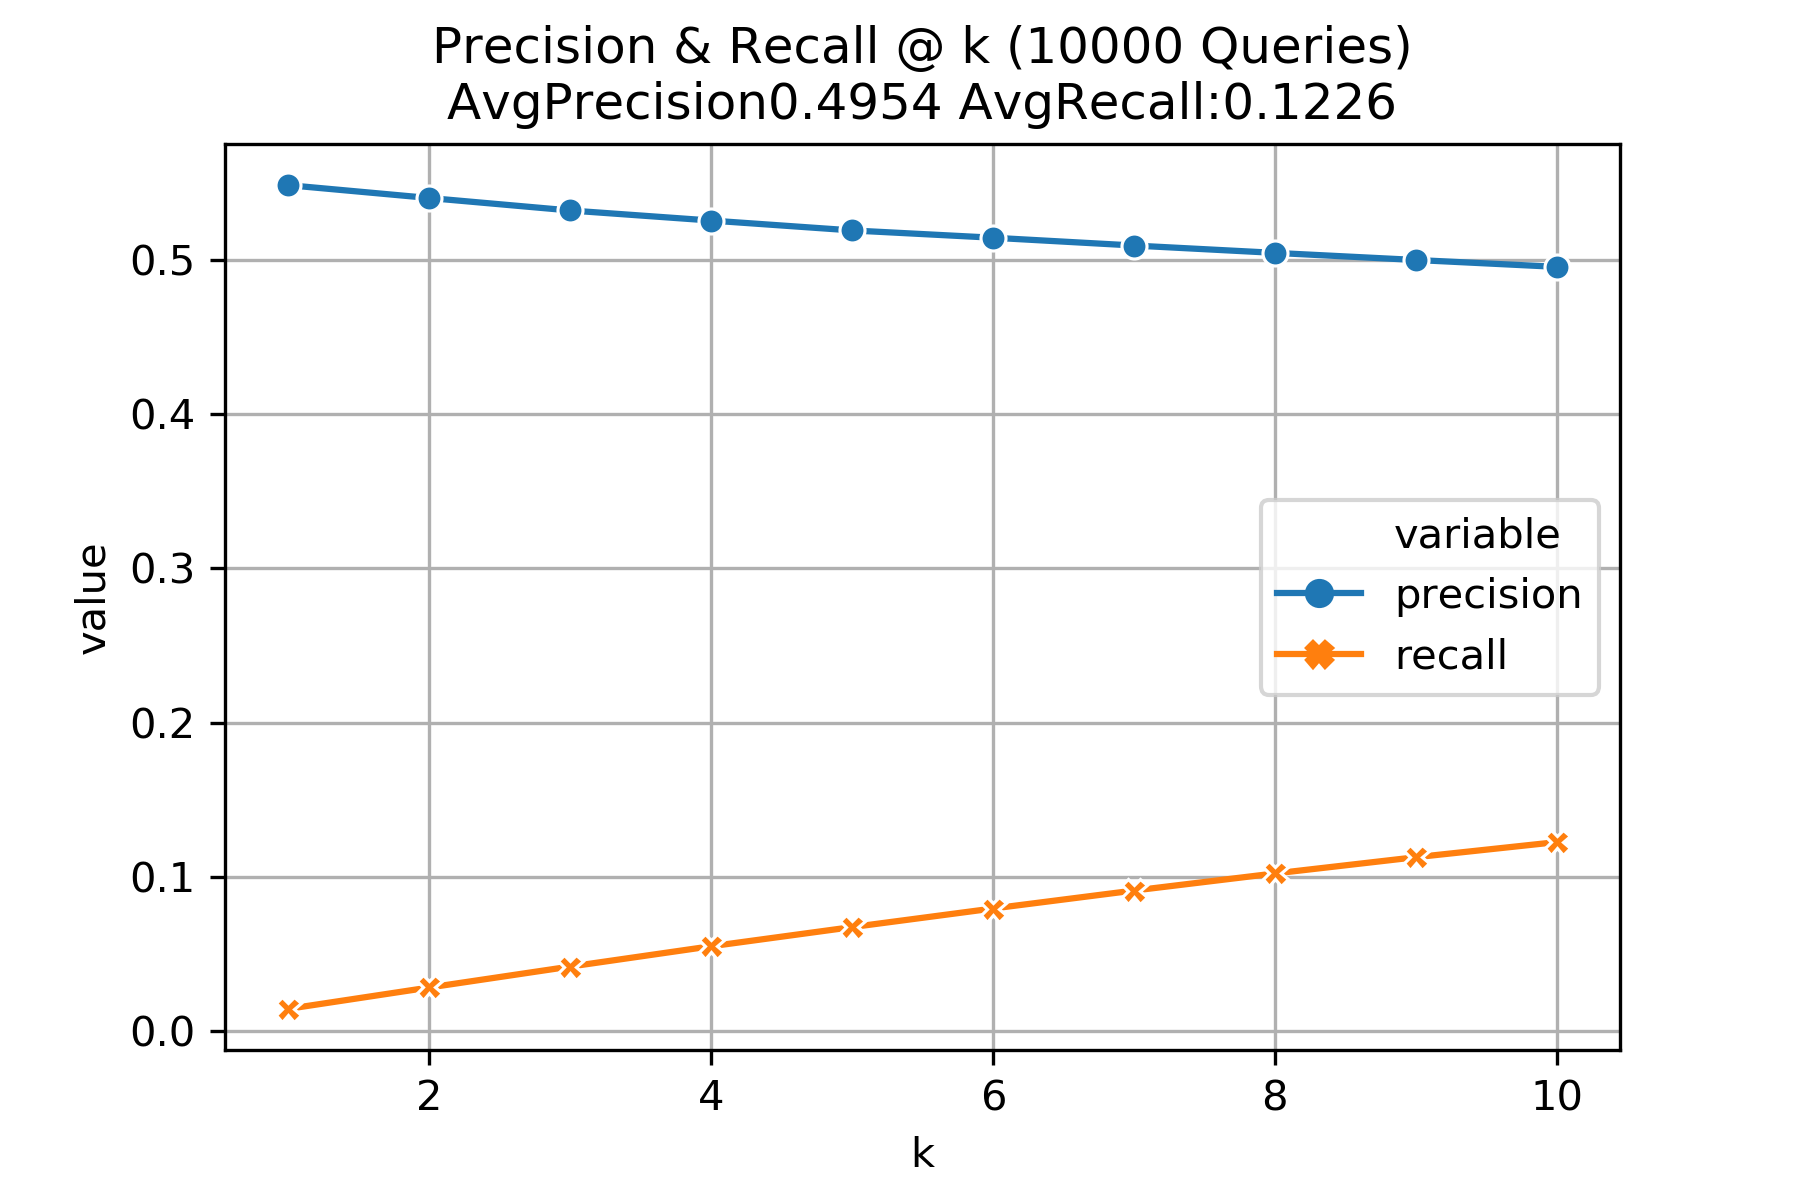
\includegraphics[scale=0.5]{fig/Precision-&-Recall-@-k-(10000-Queries).png}
		\caption{对文档内容和标题都进行匹配的检索Precision和Recall\label{fig:titleandcontent}}
	\end{minipage}

\end{figure}

从图中可以看到,就Precision和Recall来看,对标题和内容都进行匹配比只匹配文档内容得到的结果更好。对标题和内容都匹配时,索引系统的Precision@10可以达到49.54\%,Recall@10可以达到12.26\%。

就Precision和Recall的数字而言,这个两个指标并非足够优秀,但是从实际表现来看,我们的检索效果可以较好地满足需求。我们仔细分析了其中的原因,认为测评指标低和实际效果好并不矛盾,这是由于我们采用了有13000000+篇文档的DuReader数据集。

从Precision来看,DuReader数据集内容涵盖广,对于一个特定的问题,检索到的与该问题相关的文档可能在另一个问题的相关文档中,从而导致Precision从数值上较低,但由于文档数量多,对各种各样的问题基本都有相应的解答,实际检索效果很好。

从Recall来看,DuReader数据集文档非常多,我们把每一个Paragraph都作为一个文档,导致某些问题对应的文档可能有上百个,但我们设定索引1次最多返回10篇文档,即使这10篇全部都是相关的文档,Recall仍然会较低。

\subsection{阅读理解模型}  % 戴傲初
\subsubsection{接口调用}
模型部分接口较为简洁。在后端的实际运行过程中,可以使用到的模型接口仅一个:

\begin{lstlisting}
rpc_client.get_answer_from_server(question, hit_meta, address)
\end{lstlisting}

参数解释如下:
\begin{itemize}
  \item question, str,向模型提出的问题;
  \item hit\_meta, list,其中每一项是一条文档源数据,包含文档内容、文档id、es分数等;
  \item address, str,为ip地址与port的拼接;
\end{itemize}

发送给模型之后,接口会在hit\_meta中每一项添加预测的答案、评价的分数、置信程度,以及文档中答案的起始位置和结束位置,将这一个补充的hit\_meta作为返回值。

\subsubsection{模型运行原理概述}
我们使用的是美团用户代表方面提供的预训练语言模型,进行抽取式阅读理解任务\cite{MRC-MODEL}。
\begin{figure}[H]  % htbp是插入图片的位置参数,直接用就好
    \centering  % 使图片居中
    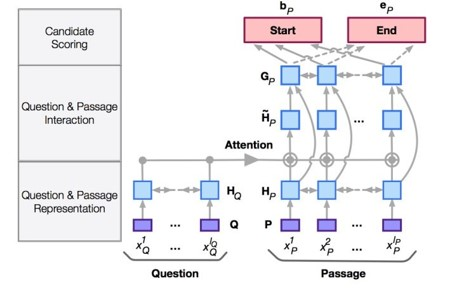
\includegraphics[width=0.5\textwidth]{fig/MRC-model.jpg}
    \caption{抽取式阅读理解}  %  图片的标题
\end{figure}
在任务中,模型得到一条问题和一篇文档,将问题与文档编码并输入给BERT模型,由模型判断出最有可能是答案的文档片段,并输出预测答案的起始位置和终止位置。

在实际的使用过程中,模型被封装为一个对象实例\textbf{mrc\_module},其中的fit函数可以接收若干篇文档与一个问题,分别对每一篇文档进行预测,返回相应的答案。该函数为我们实际使用的函数。

为了把握模型运行速度,我们控制了每次发送的文档数量与文档平均长度变量,监控模型若干次得到答案的平均时间,如下:
\begin{figure}[H]  % htbp是插入图片的位置参数,直接用就好
    \centering  % 使图片居中
    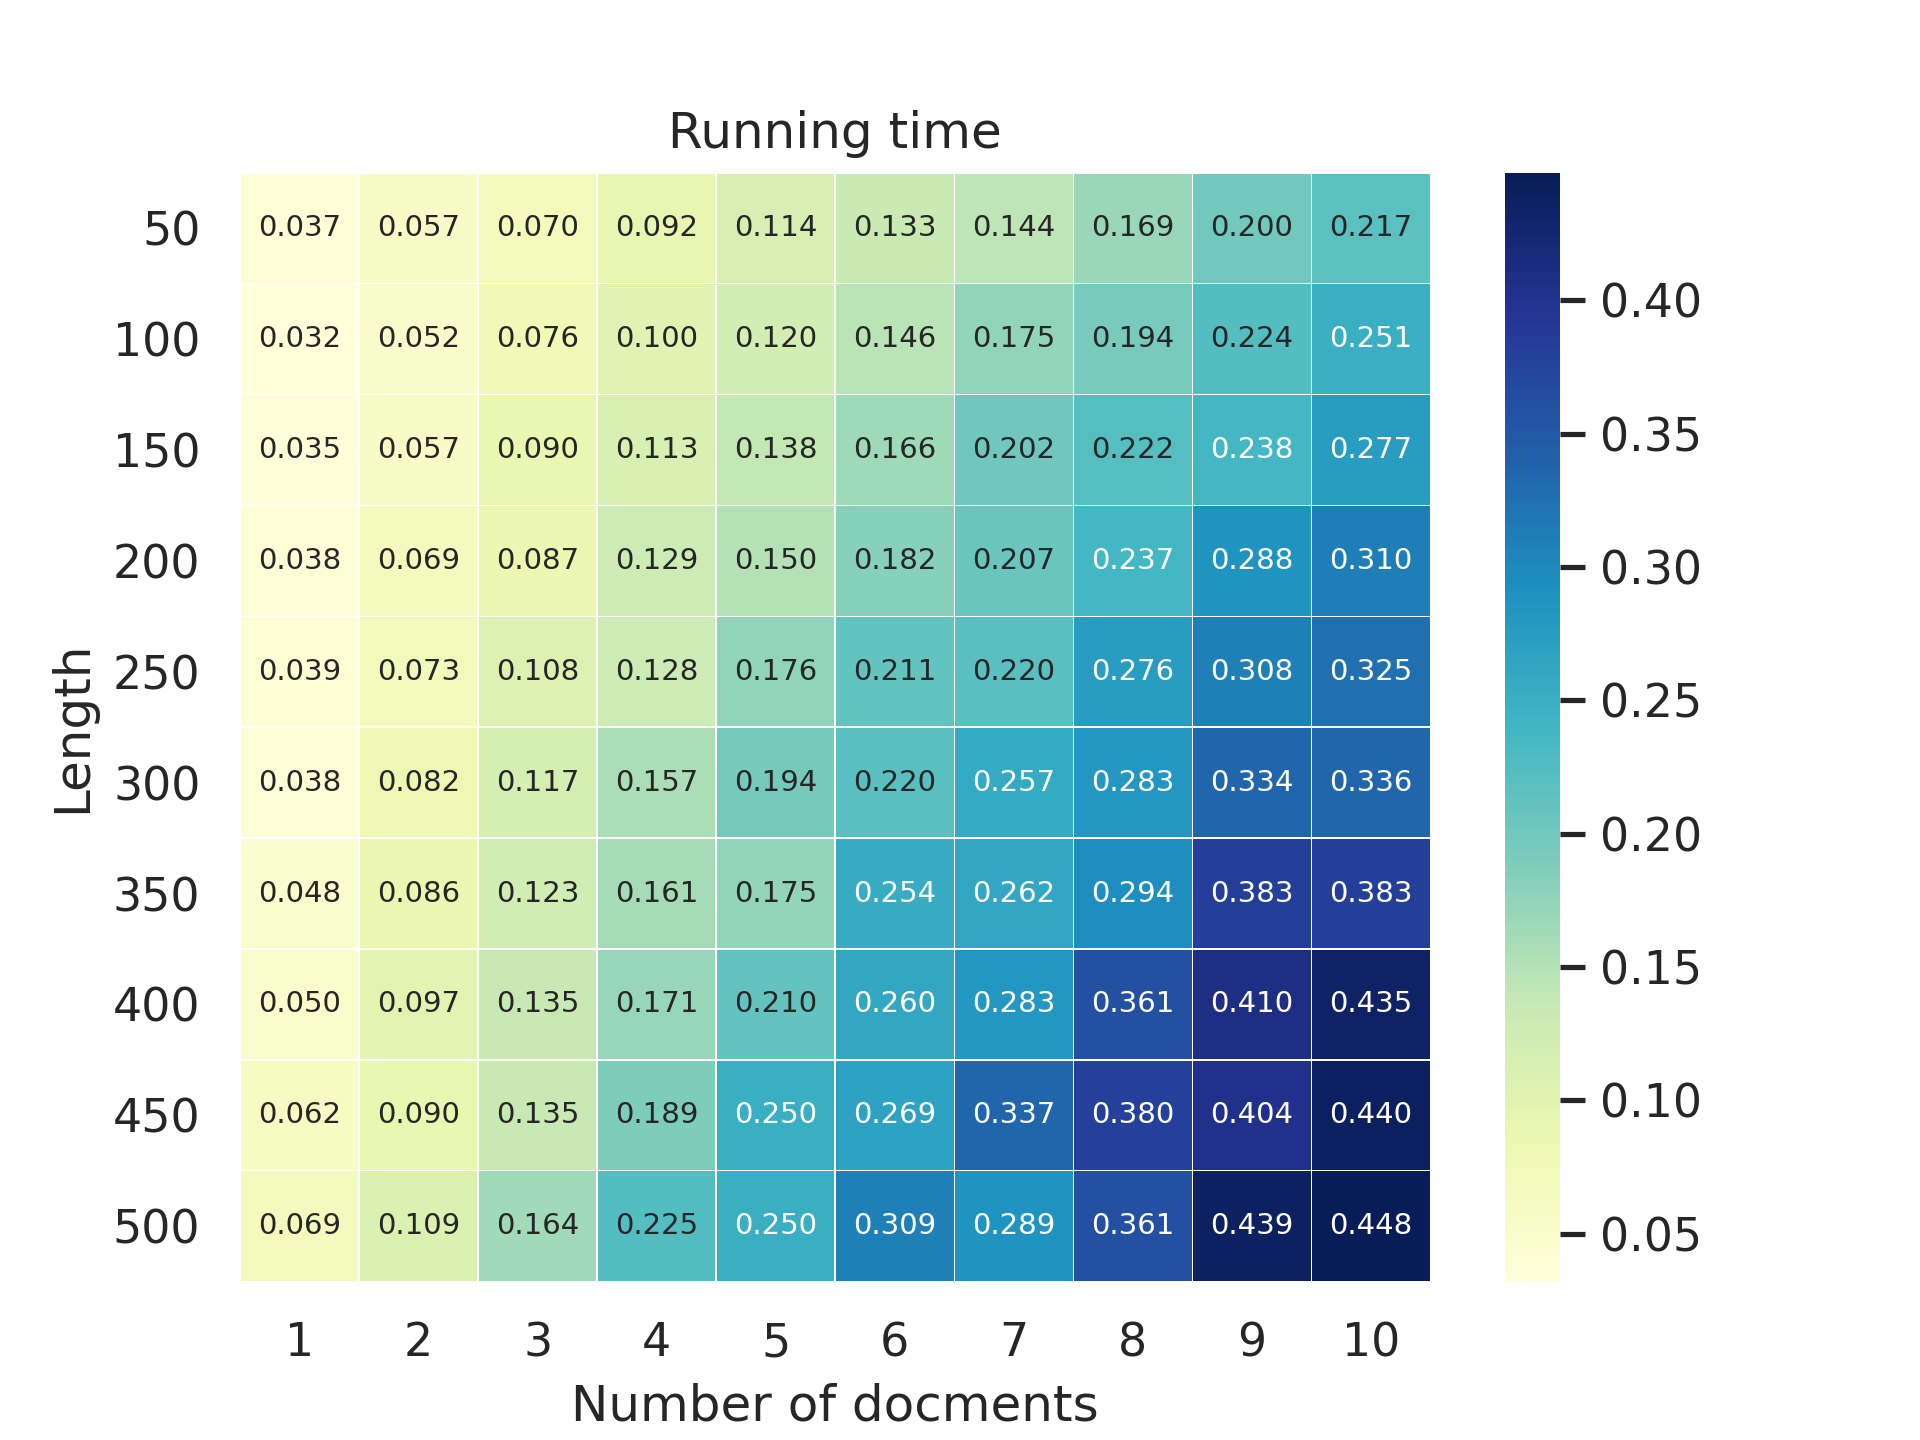
\includegraphics[width=0.5\textwidth]{fig/remote.png}
    \caption{模型时间评测}  %  图片的标题
\end{figure}
可以看到,在控制10篇文档,且文档平均长度在500字以下时,模型可以在0.4s左右得到答案。实际上线的Dureader数据集,文档长度往往不足100字,故返回速度较为可观。

\subsubsection{部署}
预训练语言模型对算力的要求较高,故我们需要将模型主体部分在GPU服务器上进行部署。服务器目前的配置为:Tesla T4显卡一块,cuda版本11.1,以及若干额外优化操作:

\textbf{apex}:nvidia提供的开源混合精度计算框架。它可以动态选择模型中参数为fp16或fp32,可以降低显存开销、提高训练速度。

\textbf{cudnn}:NVIDIA cuDNN是用于深度神经网络的GPU加速库。它强调性能、易用性和低内存开销,可以集成到更高层次的机器学习框架中。它的代码实现是插入式的,即可以在不更改原先代码框架的情况下进行优化。

此外,在云服务器上存在着模型的两个版本,即cmrc版本和dureader版本,可以进行便捷的切换与调试。

\subsubsection{通信}
我们采用了远程过程调用机制(RPC)实现腾讯云端与django后端的通信。具体地,当django后端需要进行通信时,会向腾讯云端发送一个确定的函数运行指令,与一个xml格式的字符串。同时云端会在固定端口进行监听,若得到函数运行指令,就执行相应的函数、发回一个返回字符串作为回应。

例如,我们将模型的加载与预测部分写进函数\textbf{respon\_string}中,并将其注册为名称"get\_string",在模型与后端的接口处,每次发送数据时的函数运行指令即为"get\_string"。

\section{数据库设计}  % 刘畅
\subsection{数据库整体结构}
数据库中包含了九张表,如下:
% Please add the following required packages to your document preamble:
% \usepackage{multirow}
\begin{table}[h]
\caption{数据库中所有表的名称}
\centering
\begin{tabular}{|c|c|}
\hline
表名                      & 作用                                  \\ \hline
auth\_group             & \multirow{7}{*}{django admin模块自动生成} \\ \cline{1-1}
auth\_group\_permission &                                     \\ \cline{1-1}
auth\_permission        &                                     \\ \cline{1-1}
django\_admin\_log      &                                     \\ \cline{1-1}
django\_content\_type   &                                     \\ \cline{1-1}
django\_migrations      &                                     \\ \cline{1-1}
django\_session         &                                     \\ \hline
manage\_doc\_document   & 文档信息                                \\ \hline
manage\_user\_user      & 用户信息                                \\ \hline
\end{tabular}
\end{table}

\newpage
真正自行设计的只有后面两张表。

\subsection{各字段解释}
\begin{table}[h]
\caption{manage\_user\_user}
\centering
\begin{tabular}{|c|c|c|}
\hline
字段          & 数据类型    & 解释       \\ \hline
user\_id    & integer & 用户id     \\ \hline
password    & string  & 密码       \\ \hline
username    & string  & 用户名      \\ \hline
email       & string  & 邮箱       \\ \hline
created\_at & date    & 创建账户时间   \\ \hline
updated\_at & date    & 账户信息更新时间 \\ \hline
is\_delete  & bool    & 用户是否被删除  \\ \hline
is\_active  & bool    & 用户是否活跃   \\ \hline
is\_admin   & bool    & 用户是否是管理员 \\ \hline
query\_json & string  & 历史记录     \\ \hline
bio         & string  & 个人简介     \\ \hline
\end{tabular}
\end{table}
其中我自己设计了历史记录字符串的json格式,解决了数据库不方便存储数组的问题。
query\_json字段的json格式如下:
\begin{lstlisting}
{
   "data":[
      {
         "question":"question1",
         "time":1603958422.039079,
         "response":[
            {
               "answer":"answer1",
               "grade":12.07,
               "content":"content1",
               "doc_id":3516
            },
            {
               "answer":"answer2",
               "grade":12.07,
               "content":"content2",
               "doc_id":3517
            }
         ]
      }
   ]
}
\end{lstlisting}   
\begin{table}[h]
\caption{manage\_doc\_document}
\centering
\begin{tabular}{|c|c|c|}
\hline
字段      & 数据类型    & 解释   \\ \hline
id      & integer & 文档id \\ \hline
status  & integer & 文档状态 \\ \hline
content & string  & 文档内容 \\ \hline
title   & string  & 文档标题 \\ \hline
src     & integer & 文档来源 \\ \hline
\end{tabular}
\end{table}

文档表的各个字段从名字上就可以看出其意义。文档id作为表的主键,便于查找文档,文档的status用来软删除/恢复文档内容,title和content分别标志
文档的内容和标题,src代表文档的来源。其中,-1/0/1/2/3/4/5/6/7分别对应了默认值/用户上传/cmrc/\newline search.train/zhidao.train/search.dev/zhidao.dev/search.test/zhidao.test九个类别。

\section{项目感想}  % 每个人各自写
\subsection{潘传宇}
首先,感谢软件工程课程提供的开发实践机会,使得我有幸能够体验一次较为真实的软件开发流程;感谢软工课的老师和助教;当然最需要感谢的还是在本次项目中并肩作战的队友们。

从技术角度来说,虽然这是我第一次较为正式地接触前端开发,但是我发现前端的入门门槛并不算高,如果只限于调库的话,上手还是很快的。但是如果仅仅只是调库,很多期望的自定义特性就难以实现,因此还是要回到html/css/javascript的原始设计上来。前端说到底还是视觉效果,核心是好看、有视觉冲击力,因此相比技术,前端在设计方面的成分可能要更多一些。从这一角度来看,不依赖外界库从零设计好看的前端又是很难的。在我们的开发中,vue框架所提供的组件化设计以及Element-UI提供的丰富的组件都给我们的开发带来了很大的便利,但同时,在一些我们需要自主设计和修改的情境下又带来一些不便。

从协作角度来说,我认为本次我们的小组合作是无可挑剔的。无论是整体进度的安排和把控、组员的配合程度、各个阶段的完成质量都相当到位,最终我们也做出了不错的效果。这让我深刻认识到了,一个优秀的团队不一定需要每个队员的个人能力都特别优秀,但一定需要团队中的每个人有一致的动机、足够的投入、充分的交流。

不得不说,这是一次很难得也很开心的经历,尤其是和这么一些靠谱的队友一起完成一件有意义的事。希望日后有机会再次合作,再创佳绩!

\subsection{邹恬圆}
这次软工项目的合作非常舒适,能感受到无论是组长还是小组成员都有在认真的对待分给自己的任务。我们应该是开会最频繁的一个软工小组,前4个sprint里每周都会有两到三次的全组会。紧锣密鼓的会议、同伴的相互督促,使得我们整个项目的推进进度非常可人。但个人认为,此项目最大的问题在于项目细节逻辑不够严谨,例如前后端通信的安全性保证、前端用户不合法操作的过滤都没有考虑得非常周全。这是未来我们真正在开发项目时需要注意的地方。

同时,在这次合作中我也从队友的身上学到了很多:一起负责前端的队友活学活用地用fong模型渲染完成炫酷的Home页面设计;负责数据库的同学令人惊叹、令人折服地完成了多次几十G数据库迁移;负责模型的同学细致灵活地运用各种手段解决用户代表提供的模型中的小bug;负责整体调度安排的组长令人叹服地长期保持着极大的项目热情。

整个项目中给我印象最深刻的莫过于前端Element-UI组件的使用。一句话概括使用体验就是“使用Element-UI,构建功能正确的页面需要10分钟,美化界面、微调组件功能到符合大众需求需要10小时”。我这段时间发现,这也是我身边的同学们在使用各种轮子的普遍感受。这激励着我在未来更加积极地为开源社区提供问题反馈甚至提供改进方案和代码。

项目即将全面结束,感谢这一路上多位课程助教的大力支持,感谢同项目的各位同学之间项目的技术栈支持,感谢强大队友的认真付出。

\subsection{刘畅}
软工作为贵系大三上课程的重头戏,本以为开发过程会十分刺激和紧张,但实际上整体开发节奏却把握得非常好,我觉得相当一部分原因在于负责队长的及时沟通、推进和靠谱队友们的通力合作,这个过程中我也得到了非常良好的开发体验,并且学习到了很多技术之外的东西。

就我个人而言,本次开发过程中的技术栈主要集中在后端框架、数据库和后端单元测试上。实话说,这部分内容除了需要学习环境的配置以及诸如Pytest这类工具如何使用上,似乎并不需要学习很多额外的东西。主要时间还是花在了如何迁移数据库以及调试代码逻辑、写单元测试上了,尤其是项目后期快要收工时,我还是克服了重重困难,利用Docker技术在项目服务器上配置好了MySQL环境,并将我们最后一版数据集内容装载到了数据库中。这个过程少不了队友们的鼓励和助教们的帮助!

另外,因为负责项目的API部分,所以在进行joint testing的时候我的一些疏忽经常导致项目功能上线延迟。让前端和后端的其他队友被迫进行等待。我十分惭愧,同时也认识到了要成为一名合格的后端工程师,写出高鲁棒性的代码是相当重要的,能给整个团队节约很多时间。

还有一点感想。我们平常所认为的很容易的问题,当更换了新的场景之后可能变得非常困难。就拿数据库来说,当数据量增大、用户数增多、并发性要求变高的时候,现有的框架可能需要进行更改甚至被弃用。因此一名好的软件架构师应该在充分理解需求的基础上进行选择和软件结构的设计,同时也要慢慢学会从特定场景出发,自己造轮子,为解决业界问题做出自己的贡献。

最后还是要感谢软工课程团队提供的相应指导和资源支持,感谢美团对本次大作业提供的技术支持,感谢队友们的鼓励和信任,相信这学期的训练能够对我们今后的开发生涯有深远影响。

\subsection{戴傲初}
技术上,我在本次软工项目中负责了阅读理解模型方面的工作。经过实践,我掌握并熟练了环境配置、代码阅读、代码重构、代码部署等策略,并对工业界相关软件的人工智能内核运行方式有了一定的了解。此外,完善的项目合作让我始终对队友们的工作保持了解,并能通过版本控制等方法协同合作解决问题。

过程上,我们的软工项目具有明确的时间规划与行动细节。队长热心负责、要求明确,队友勇于拓展、行动力强。在我所了解的软工小队中,我们小组可以说是最具有软工思想、符合软件工程要求的一个团队之一了。

情感上,这次组队任务是我在大学期间体验感最良好的一次合作项目。与队友建立深厚友情的同时,我认识并改进了自己的不足之处,收获颇丰。

\subsection{任一}
本项目作为一个软工项目,可以说是较为成功的。项目的顺利完成,离不开各位同学在项目上的投入,也离不开老师、助教的悉心指导和关注。

从我自己来说,这是我作为Team Leader的又一次锻炼,这也是我非常用心组织的一个团队,最终效果不错也令我很开心。每次开会前我都会有一定的心理压力,准备会议提纲,统筹项目进度,尽力照顾到每个同学的感受,我认为这些都是做一个成熟的Team Leader所必要的素质,我在整个项目的统筹中也学习到了许多。

从技术上来说,整个团队的技术水平都很高,各位通力合作,实现了$1 \times 5 > 5$的效果。我们在开发的过程中,也努力将软件工程的精神和技术贯穿始终,用科学合理的方法开发整个系统。

但本次项目也有一些不足,例如安全性方面,无论是前后端的通信,还是后端对索引、模型的调用,都存在一定的安全隐患。出于课程时间的紧张,很多小细节我们并没有完善好,这也是在实际开发中需要注意的。

年轻人,前程似海,来日方长。通过本次软件工程项目的学习和锻炼,我收获良多。祝团队里的成员未来可期,我们有缘再会。也祝帮助过我们的老师、助教和同学们,身体健康、工作顺利!

\bibliographystyle{plain}  % 引用风格是plain
\bibliography{ref}  % 这里的这个ref就是对文件ref.bib的引用

\end{document}
